% !TeX root = main.tex
%%%%%%%%%%%%%%%%%%%%%%%%%%%%%%%%%%%%%%%%%
% kaobook
% LaTeX Template
% Version 1.2 (4/1/2020)
%
% This template originates from:
% https://www.LaTeXTemplates.com
%
% For the latest template development version and to make contributions:
% https://github.com/fmarotta/kaobook
%
% Authors:
% Federico Marotta (federicomarotta@mail.com)
% Based on the doctoral thesis of Ken Arroyo Ohori (https://3d.bk.tudelft.nl/ken/en)
% and on the Tufte-LaTeX class.
% Modified for LaTeX Templates by Vel (vel@latextemplates.com)
%
% License:
% CC0 1.0 Universal (see included MANIFEST.md file)
%
%%%%%%%%%%%%%%%%%%%%%%%%%%%%%%%%%%%%%%%%%

%----------------------------------------------------------------------------------------
%	PACKAGES AND OTHER DOCUMENT CONFIGURATIONS
%----------------------------------------------------------------------------------------

\documentclass[
	fontsize=10pt, % Base font size
	twoside=false, % Use different layouts for even and odd pages (in particular, if twoside=true, the margin column will be always on the outside)
	%open=any, % If twoside=true, uncomment this to force new chapters to start on any page, not only on right (odd) pages
	%chapterprefix=true, % Uncomment to use the word "Chapter" before chapter numbers everywhere they appear
	%chapterentrydots=true, % Uncomment to output dots from the chapter name to the page number in the table of contents
	numbers=noenddot, % Comment to output dots after chapter numbers; the most common values for this option are: enddot, noenddot and auto (see the KOMAScript documentation for an in-depth explanation)
	%draft=true, % If uncommented, rulers will be added in the header and footer
	%overfullrule=true, % If uncommented, overly long lines will be marked by a black box; useful for correcting spacing problems
]{kaobook}
%!TEX root = ../thesis.tex

%\hypersetup{colorlinks,linktocpage,urlcolor=red}
%
%\definecolor{myGreen}{HTML}{05C18E} 
%\definecolor{myGreenDarker}{HTML}{178C6C} \colorlet{mylinkcolor}{green!50!black}

\definecolor{webbrown}{rgb}{.6,0,0}

\hypersetup{
  colorlinks=true,
  linkcolor=black, %myGreenDarker
%  urlcolor=myGreenDarker,
  citecolor = webbrown,
  urlcolor=webbrown,
  hyperfootnotes=false,
  hypertexnames,
  bookmarks=true}
  
%\setsidenotefont{\color{black}\footnotesize}   <-- set the color and font here
%\setmarginnotefont{\color{black}\footnotesize} <-- and here
%
%\renewcommand{\maketitlepage}[0]{%
%  \cleardoublepage%
%  {%
%  \sffamily%
%  \begin{fullwidth}%
%  \fontsize{18}{20}\selectfont\par\noindent\textcolor{darkgray}{\allcaps{\thanklessauthor}}%
%  \vspace{11.5pc}%
%  \fontsize{24}{45}\selectfont\par\noindent\textcolor{darkgray}{\allcaps{\thanklesstitle}}
%  \fontsize{17.4}{25}\selectfont\par\noindent\textcolor{darkgray}{\allcaps{For Affective Touch Communication}}%
%  \fontsize{10.0}{17}\selectfont\par\noindent\textcolor{Gray}{\allcaps{Devices that touch to convey emotions and feel that contact}}%
%
%  \vfill%
%  \fontsize{14}{16}\selectfont\par\noindent\allcaps{\thanklesspublisher}%
%  \end{fullwidth}%
%  }
 %  \thispagestyle{empty}%
%  \clearpage%
%}

%%%% Kevin Godny's code for title page and contents from https://groups.google.com/forum/#!topic/tufte-latex/ujdzrktC1BQ
% \makeatletter
% \renewcommand{\maketitlepage}{%
% \begingroup%
% \setlength{\parindent}{0pt}

% {\fontsize{24}{24}\selectfont\textit{\@author}\par}

% \vspace{1.75in}{\fontsize{36}{54}\selectfont\@title\par}

% % \vspace{0.5in}{\fontsize{14}{14}\selectfont\textsf{\smallcaps{\@date}}\par}
% \vspace{0.5in}{\fontsize{14}{14}\selectfont\textsf{\sc\@date}\par}

% \vfill{\fontsize{14}{14}\selectfont\textit{\@publisher}\par}

% \thispagestyle{empty}
% \endgroup
% }
% \makeatother

%\titlecontents{part}%
%    [0pt]% distance from left margin
%    {\addvspace{0.25\baselineskip}}% above (global formatting of entry)
%    {\allcaps{Part~\thecontentslabel}\allcaps}% before w/ label (label = ``Part I'')
%    {\allcaps{Part~\thecontentslabel}\allcaps}% before w/o label
%    {}% filler and page (leaders and page num)
%    [\vspace*{0.5\baselineskip}]% after
%
%
%\titlecontents{chapter}%
%    [4em]% distance from left margin
%    {}% above (global formatting of entry)
%    {\contentslabel{2em}\textit}% before w/ label (label = ``Chapter 1'')
%    {\hspace{0em}\textit}% before w/o label
%    {\qquad\thecontentspage}% filler and page (leaders and page num)
%    [\vspace*{0.5\baselineskip}]% after
%%%%% End additional code by Kevin Godby


%% CHANGE CITE COMMAND
\renewcommand{\cite}[1]{%
~\citep{#1}%
}



%%
% If they're installed, use Bergamo and Chantilly from www.fontsite.com.
% They're clones of Bembo and Gill Sans, respectively.
%\IfFileExists{bergamo.sty}{\usepackage[osf]{bergamo}}{}% Bembo
%\IfFileExists{chantill.sty}{\usepackage{chantill}}{}% Gill Sans

%%%%%%%%%%%%%%%%%%%%%%%%%%%%%%%%%%%%%%%%%%%%%%%%%%%%%%%%%%
%%% INCLUSION / EXCLUSION %%%%%%%%%%%%%%%%%%%
\usepackage{microtype}
\usepackage{comment}
% !!! Comment or uncomment line under to exclude or include the content of the chapter:
%\excludecomment{content} % exclude the content, (only get introduction and summary)
\includecomment{content} % include the content, (get eveevolutionrything)
\includecomment{export}
%%%%%%%%%%%%%%%%%%%%%%%%%%%%%%%%%%%%%%%%%%%%%%%%%%%%%%%%%%


%%
% For nicely typeset tabular material
\usepackage{booktabs}
%%
% For graphics / images
\usepackage{graphicx}
\setkeys{Gin}{width=\linewidth,totalheight=\textheight,keepaspectratio}
\graphicspath{{graphics/}}
% The fancyvrb package lets us customize the formatting of verbatim environments.  We use a slightly smaller font.
\usepackage{fancyvrb}
\fvset{fontsize=\normalsize}

%%
% Prints argument within hanging parentheses (i.e., parentheses that take
% up no horizontal space).  Useful in tabular environments.
% \newcommand{\hangp}[1]{\makebox[0pt][r]{(}#1\makebox[0pt][l]{)}}

%%
% Prints an asterisk that takes up no horizontal space.
% Useful in tabular environments.
% \newcommand{\hangstar}{\makebox[0pt][l]{*}}

%%
% Prints a trailing space in a smart way.
\usepackage{xspace}

%
%%%
%% Some shortcuts for Tufte's book titles.  The lowercase commands will
%% produce the initials of the book title in italics.  The all-caps commands
%% will print out the full title of the book in italics.
%\newcommand{\vdqi}{\textit{VDQI}\xspace}
%\newcommand{\ei}{\textit{EI}\xspace}
%\newcommand{\ve}{\textit{VE}\xspace}
%\newcommand{\be}{\textit{BE}\xspace}
%%\newcommand{\VDQI}{\textit{Visualizing dynamic social data  with rationally designed constructive systems}\xspace}
%\newcommand{\EI}{\textit{Envisioning Information}\xspace}
%\newcommand{\VE}{\textit{Visual Explanations}\xspace}
%\newcommand{\BE}{\textit{Beautiful Evidence}\xspace}
%\newcommand{\TL}{Tufte-\LaTeX\xspace}

% Prints the month name (e.g., January) and the year (e.g., 2008)
% \newcommand{\monthyear}{%
%   \ifcase\month\or January\or February\or March\or April\or May\or June\or
%   July\or August\or September\or October\or November\or
%   December\fi\space\number\year
% }





% Prints an epigraph and speaker in sans serif, all-caps type.
\newcommand{\openepigraph}[2]{%
  %\sffamily\fontsize{14}{16}\selectfont
  \begin{fullwidth}
  \sffamily\large
  \begin{doublespace}
  \noindent\allcaps{#1}\\% epigraph
  \noindent\allcaps{#2}% author
  \end{doublespace}
  \end{fullwidth}
}

% Inserts a blank page
% \newcommand{\blankpage}{\newpage\hbox{}\thispagestyle{empty}\newpage}

\usepackage{units}

% Typesets the font size, leading, and measure in the form of 10/12x26 pc.
\newcommand{\measure}[3]{#1/#2$\times$\unit[#3]{pc}}

% Macros for typesetting the documentation
\newcommand{\hlred}[1]{\textcolor{Green}{#1}}% prints in red
\newcommand{\hangleft}[1]{\makebox[0pt][r]{#1}}
% \newcommand{\hairsp}{\hspace{1pt}}% hair space
\newcommand{\hquad}{\hskip0.5em\relax}% half quad space
\newcommand{\TODO}{\textcolor{red}{\bf TODO!}\xspace}
% \newcommand{\ie}{\textit{i.\hairsp{}e.}\xspace}
% \newcommand{\eg}{\textit{e.\hairsp{}g.}\xspace}
% \newcommand{\na}{\quad--}% used in tables for N/A cells
\providecommand{\XeLaTeX}{X\lower.5ex\hbox{\kern-0.15em\reflectbox{E}}\kern-0.1em\LaTeX}
\newcommand{\tXeLaTeX}{\XeLaTeX\index{XeLaTeX@\protect\XeLaTeX}}
% \index{\texttt{\textbackslash xyz}@\hangleft{\texttt{\textbackslash}}\texttt{xyz}}
\newcommand{\tuftebs}{\symbol{'134}}% a backslash in tt type in OT1/T1
\newcommand{\doccmdnoindex}[2][]{\texttt{\tuftebs#2}}% command name -- adds backslash automatically (and doesn't add cmd to the index)
\newcommand{\doccmddef}[2][]{%
  \hlred{\texttt{\tuftebs#2}}\label{cmd:#2}%
  \ifthenelse{\isempty{#1}}%
    {% add the command to the index
      \index{#2 command@\protect\hangleft{\texttt{\tuftebs}}\texttt{#2}}% command name
    }%
    {% add the command and package to the index
      \index{#2 command@\protect\hangleft{\texttt{\tuftebs}}\texttt{#2} (\texttt{#1} package)}% command name
      \index{#1 package@\texttt{#1} package}\index{packages!#1@\texttt{#1}}% package name
    }%
}% command name -- adds backslash automatically
\newcommand{\doccmd}[2][]{%
  \texttt{\tuftebs#2}%
  \ifthenelse{\isempty{#1}}%
    {% add the command to the index
      \index{#2 command@\protect\hangleft{\texttt{\tuftebs}}\texttt{#2}}% command name
    }%
    {% add the command and package to the index
      \index{#2 command@\protect\hangleft{\texttt{\tuftebs}}\texttt{#2} (\texttt{#1} package)}% command name
      \index{#1 package@\texttt{#1} package}\index{packages!#1@\texttt{#1}}% package name
    }%
}% command name -- adds backslash automatically
\newcommand{\docopt}[1]{\ensuremath{\langle}\textrm{\textit{#1}}\ensuremath{\rangle}}% optional command argument
\newcommand{\docarg}[1]{\textrm{\textit{#1}}}% (required) command argument
\newenvironment{docspec}{\begin{quotation}\ttfamily\parskip0pt\parindent0pt\ignorespaces}{\end{quotation}}% command specification environment
\newcommand{\docenv}[1]{\texttt{#1}\index{#1 environment@\texttt{#1} environment}\index{environments!#1@\texttt{#1}}}% environment name
\newcommand{\docenvdef}[1]{\hlred{\texttt{#1}}\label{env:#1}\index{#1 environment@\texttt{#1} environment}\index{environments!#1@\texttt{#1}}}% environment name
\newcommand{\docpkg}[1]{\texttt{#1}\index{#1 package@\texttt{#1} package}\index{packages!#1@\texttt{#1}}}% package name
\newcommand{\doccls}[1]{\texttt{#1}}% document class name
\newcommand{\docclsopt}[1]{\texttt{#1}\index{#1 class option@\texttt{#1} class option}\index{class options!#1@\texttt{#1}}}% document class option name
\newcommand{\docclsoptdef}[1]{\hlred{\texttt{#1}}\label{clsopt:#1}\index{#1 class option@\texttt{#1} class option}\index{class options!#1@\texttt{#1}}}% document class option name defined
\newcommand{\docmsg}[2]{\bigskip\begin{fullwidth}\noindent\ttfamily#1\end{fullwidth}\medskip\par\noindent#2}
\newcommand{\docfilehook}[2]{\texttt{#1}\index{file hooks!#2}\index{#1@\texttt{#1}}}
\newcommand{\doccounter}[1]{\texttt{#1}\index{#1 counter@\texttt{#1} counter}}




%\geometry{textwidth=.55\paperwidth}


% Generates the index
\usepackage{makeidx}
\makeindex



% Nomenclature
%\usepackage{nomencl}
%\renewcommand{\nomname}{List of Abbreviations}
%\makenomenclature



%%%%
\makeatletter
\renewcommand*\l@figure{\@dottedtocline{1}{1.5em}{2.3em}}
\makeatother

%% change TOC
\setcounter{tocdepth}{2}
\setcounter{secnumdepth}{2}

%%%%%%%%%%%%%%%%%%%%%%%%%%%%%%%%%%%%%%%%%%%%%%%%%%
%%%%%%%%%%%%%%%%%%%%%%%%%%%%%%%%%%%%%%%%%%%%%%%%%%
\usepackage{amssymb}% http://ctan.org/pkg/amssymb
\usepackage{pifont}% http://ctan.org/pkg/pifont
%\usepackage{graphics} % for EPS, load graphicx instead
\usepackage{graphicx}
\usepackage{multirow}
\usepackage{xspace}
\usepackage{tabularx}
\usepackage{color}
\usepackage{listings}
\usepackage[normalem]{ulem}
\usepackage{colortbl}
\usepackage{morefloats}
\usepackage{enumitem}
\usepackage{rotating}
\usepackage{comment}
\usepackage{rotating}
% \usepackage[sort, numbers]{natbib} 
\usepackage[retainorgcmds]{IEEEtrantools}
\usepackage{bibentry}
\usepackage{longtable}
\usepackage{glossaries}
\usepackage{gensymb}
\usepackage{csvsimple}
\usepackage{amsmath}
\usepackage{cleveref}% Has to be loaded after hyperref
\usepackage[utf8]{inputenc}
\usepackage{todonotes}
\usepackage{marginfix}
\usepackage[export]{adjustbox}
\usepackage{fullwidth}
%\setkeys{Gin}{height=2cm}
%\usepackage{float}
\usepackage[caption=false]{subfig}

\usepackage[strict]{changepage}

\setlist[description]{style = multiline, labelwidth = 55pt}
\usepackage[parfill]{parskip}
\makeatletter
% Paragraph indentation and separation for normal text
% \renewcommand{\@tufte@reset@par}{%
%   \setlength{\RaggedRightParindent}{1.0pc}%
%   \setlength{\parindent}{1pc}%
%   \setlength{\parskip}{8pt}%\baselineskip % default 12pt for 10pt font
% }
% \@tufte@reset@par

% Paragraph indentation and separation for marginal text
% \renewcommand{\@tufte@margin@par}{%
%   \setlength{\RaggedRightParindent}{0.5pc}%
%   \setlength{\JustifyingParindent}{0.0pc}%
%   \setlength{\parindent}{0.5pc}%
%   \setlength{\parskip}{6pt}%
% }
\makeatother





%% Correction

%\newcommand{\Ssubsection}[1]{{\setlength{\parindent}{0cm}\normalfont{\textit{\newline#1}}}\newline}
%\newcommand{\Ssubsection}[1]{{\setlength{\parindent}{0cm}\normalfont{\textit{#1}}}}




\usepackage{mdframed}
\newmdenv[
  leftmargin = 0pt,
  innerleftmargin = 1em,
  innerrightmargin = 0pt,
 innerbottommargin = 0pt,
  innertopmargin = 0pt,
  rightmargin = 0pt,
  linewidth = 2pt,
  topline = false,
  rightline = false,
  bottomline = false,
  skipabove = 6pt
  ]{leftbar}


\newcommand{\mframe}[1]{\begin{leftbar}{#1}\end{leftbar}}


%You can copy those commands to the preamble of your document and fill in the values that you prefer (e.g., 0pt for the indents and \baselineskip for the \parskip).








% \titleclass{\subsubsection}{straight}
% \titleformat{\subsubsection}%
%   [hang]% shape
%   {\normalfont\large\itshape}% format applied to label+text
%   {\thesubsubsection}% label
%   {1em}% horizontal separation between label and title body
%   {}% before the title body
%   []% after the title body
  
  
  

%%%%%%%%%%%%%%%%%%%%%%%%%%%%%%%%%%%%%
%%%%%% FANCY FRAMES
%% https://tex.stackexchange.com/questions/348501/example-of-box-inside-box
%%%%%%%%%%%%%%%%%%%%%%%%
%\usepackage[margin=0.5in]{geometry}
%\usepackage{tikz,lipsum,lmodern}
\usepackage{tikz,lipsum}
\usepackage[most]{tcolorbox}

\tcbset{titre/.style={boxed title style={boxrule=0pt,colframe=white}}}

\definecolor{gradientGreenL}{HTML}{1fe2ad} 
\definecolor{gradientGreenR}{HTML}{d4eb6f} 


\newtcolorbox{BoxResume}[2][]{
                boxrule=0.5pt,
                colback=white,
                top=3pt,bottom=2pt,left=2pt,right=2pt,
                colframe=webbrown,
                fonttitle=\sffamily\small,%\bfseries
                coltitle=black,
                colbacktitle=white,
                enhanced,
                attach boxed title to top left={xshift=5mm, yshift=-2mm},
                title=#2,#1
                }


\newtcolorbox{BoxIn}{
enhanced,
colframe=white,
interior style={
left color=gradientGreenL!7!white,
right color=gradientGreenR!7!white},
%frame style image=background\aa.jpg
left=5mm,
top=4mm,
bottom=4mm,
right=5mm,
boxsep=0mm,
nobeforeafter}



\newtcolorbox{BoxResumeNew}[2][]{
                boxrule=1pt,
                colback=white,
                top=3pt,bottom=2pt,left=2pt,right=2pt,
                colframe=black,
                fonttitle=\sffamily\small,%\bfseries
                coltitle=black,
                colbacktitle=white,
                enhanced,
                attach boxed title to top left={xshift=5mm, yshift=-2mm},
                title=#2,#1
                }


\newtcolorbox{BoxInNew}{
enhanced,
colframe=white,
colback=black!2!white,
%frame style image=background\aa.jpg
left=5mm,
top=4mm,
bottom=4mm,
right=5mm,
boxsep=0mm,
nobeforeafter}



\newcommand{\remember}[1]{
\vspace*{\fill}
\begin{BoxResumeNew}[titre]{WHAT YOU MUST REMEMBER}
 \begin{BoxInNew}{}
 #1
 \end{BoxInNew}{}
\end{BoxResumeNew}
\vspace{0.5cm}
} 

%%%% USAGE

%\remember{
%\textit{Contributions:}\vspace{0.5em}
%\begin{itemize}
%\item[$-$] Design and development of a finger robotic actuator for mobile devices
%\item[$-$] Applications and scenarios that demonstrate its use as a medium,  as a tool and as a virtual partner
%\item[$-$] Initial evaluation of perception of the appearance and the relevance of scenarios
%\end{itemize}
%}


%%%%%%%%%%%%%%%%%%%%%%%%%%%%%%
%%%%%%%%%   QUOTE %%%%%%%%%%%%%%%%%%%
%%%%%%%%%%%%%%%%%%

\makeatletter
\renewcommand{\@chapapp}{}% Not necessary...
\newenvironment{chapquote}[2][2em]
  {\setlength{\@tempdima}{#1}%
   \def\chapquote@author{#2}%
   \parshape 1 \@tempdima \dimexpr\textwidth-2\@tempdima\relax%
   }
  {\par\normalfont\hfill--\ \chapquote@author\hspace*{\@tempdima}\par\bigskip}
\makeatother


%\listfiles

% Set the language
\usepackage[english]{babel} % Load characters and hyphenation
\usepackage[english=british]{csquotes} % English quotes

% Load packages for testing
\usepackage{blindtext}
%\usepackage{showframe} % Uncomment to show boxes around the text area, margin, header and footer
%\usepackage{showlabels} % Uncomment to output the content of \label commands to the document where they are used


\lstset{
    language=Python, % Language
    basicstyle=\ttfamily\footnotesize, % Font style
    keywordstyle=\color{blue}\ttfamily,
    stringstyle=\color{red}\ttfamily,
    commentstyle=\color{gray}\ttfamily\itshape,
    showstringspaces=false,
    breaklines=true, % Automatic line breaking
    tabsize=4, % Tab size
    numbers=left, % Line numbers
    numberstyle=\tiny\color{gray}, % Line number style
    stepnumber=1, % Line number increment
    numbersep=5pt, % Line number separation
    frame=single, % Frame around code
    framexleftmargin=5mm, % Frame margin
    captionpos=b, % Caption position
    xleftmargin=2em, % <-- Adjust horizontal spacing here
    escapeinside={\%*}{*)} % If you want to add LaTeX within your code
}

% Load the bibliography package
\usepackage{styles/kaobiblio}
\addbibresource{main.bib} % Bibliography file

% Load mathematical packages for theorems and related environments. NOTE: choose only one between 'mdftheorems' and 'plaintheorems'.
\usepackage{styles/mdftheorems}
%\usepackage{styles/plaintheorems}

\graphicspath{{examples/documentation/images/}{images/}} % Paths in which to look for images

\makeindex[columns=3, title=Alphabetical Index, intoc] % Make LaTeX produce the files required to compile the index

\makeglossaries % Make LaTeX produce the files required to compile the glossary

\makenomenclature % Make LaTeX produce the files required to compile the nomenclature

% Reset sidenote counter at chapters
%\counterwithin*{sidenote}{chapter}
% \setcounter{section}{-1}
%----------------------------------------------------------------------------------------

\newcommand{\red}[1]{\textcolor[rgb]{1, 0, 0}{#1}}
\newcommand{\problematic}{How can sensing techniques redefine our interaction with plants ?}
%% This section is for removing the 0.*** in the sections
\makeatletter
\renewcommand{\thesection}{%
  \ifnum\c@chapter<1 \@arabic\c@section
  \else \thechapter.\@arabic\c@section
  \fi
}
\makeatother
%%%%%%%%%%%%%%%%%%%%%%%%

\begin{document}
\def\title#1{\gdef\@title{#1}\gdef\THETITLE{#1}}
%----------------------------------------------------------------------------------------
%	BOOK INFORMATION
%----------------------------------------------------------------------------------------

% \titlehead{The \texttt{kaobook} class}
\subject{Master thesis}
\title{\problematic}
\subtitle{\problematic}

\author{Matthieu SEGUI}

\date{\today}

\titlehead{\centering\includegraphics[width=6cm]{images/ift_logo.png}}

\publishers{\textbf{Supervisor}\\ Clément Duhart and Marc Teyssier}


%----------------------------------------------------------------------------------------

\frontmatter % Denotes the start of the pre-document content, uses roman numerals

%----------------------------------------------------------------------------------------
%	OPENING PAGE
%----------------------------------------------------------------------------------------

% \makeatletter
% \extratitle{
% 	% In the title page, the title is vspaced by 9.5\baselineskip
% 	\vspace*{9\baselineskip}
% 	\vspace*{\parskip}
% 	\begin{center}
% 		% In the title page, \huge is set after the komafont for title
% 		\usekomafont{title}\huge\@title
% 	\end{center}
% }
% \makeatother

%----------------------------------------------------------------------------------------
%	COPYRIGHT PAGE
%----------------------------------------------------------------------------------------

% \makeatletter
% \uppertitleback{\@titlehead} % Header

% \lowertitleback{
% 	\textbf{Disclaimer}\\
% 	You can edit this page to suit your needs. For instance, here we have a no copyright statement, a colophon and some other information. This page is based on the corresponding page of Ken Arroyo Ohori's thesis, with minimal changes.

% 	\medskip

% 	\textbf{No copyright}\\
% 	\cczero\ This book is released into the public domain using the CC0 code. To the extent possible under law, I waive all copyright and related or neighbouring rights to this work.

% 	To view a copy of the CC0 code, visit: \\\url{http://creativecommons.org/publicdomain/zero/1.0/}

% 	\medskip

% 	\textbf{Colophon} \\
% 	This document was typeset with the help of \href{https://sourceforge.net/projects/koma-script/}{\KOMAScript} and \href{https://www.latex-project.org/}{\LaTeX} using the \href{https://github.com/fmarotta/kaobook/}{kaobook} class.

% 	The source code of this book is available at:\\\url{https://github.com/fmarotta/kaobook}

% 	(You are welcome to contribute!)

% 	\medskip

% 	\textbf{Publisher} \\
% 	First printed in May 2019 by \@publishers
% }
% \makeatother

%----------------------------------------------------------------------------------------
%	DEDICATION
%----------------------------------------------------------------------------------------

% \dedication{
% 	The harmony of the world is made manifest in Form and Number, and the heart and soul and all the poetry of Natural Philosophy are embodied in the concept of mathematical beauty.\\
% 	\flushright -- D'Arcy Wentworth Thompson
% }

%----------------------------------------------------------------------------------------
%	OUTPUT TITLE PAGE AND PREVIOUS
%----------------------------------------------------------------------------------------

% Note that \maketitle outputs the pages before here

% If twoside=false, \uppertitleback and \lowertitleback are not printed
% To overcome this issue, we set twoside=semi just before printing the title pages, and set it back to false just after the title pages
\KOMAoptions{twoside=semi}
\maketitle
\KOMAoptions{twoside=false}



%----------------------------------------------------------------------------------------
%	TABLE OF CONTENTS & LIST OF FIGURES/TABLES
%----------------------------------------------------------------------------------------

\begingroup % Local scope for the following commands

% Define the style for the TOC, LOF, and LOT
%\setstretch{1} % Uncomment to modify line spacing in the ToC
% \hypersetup{linkcolor=blue} % Uncomment to set the colour of links in the ToC
\setlength{\textheight}{23cm} % Manually adjust the height of the ToC pages

% Turn on compatibility mode for the etoc package
\etocstandarddisplaystyle % "toc display" as if etoc was not loaded
\etocstandardlines % toc lines as if etoc was not loaded

% Comment both of the following lines to have the LOF and the LOT on different pages
\let\cleardoublepage\bigskip
\let\clearpage\bigskip

\setcounter{tocdepth}{3}
\setcounter{secnumdepth}{3}

% \listoftables % Output the list of tables

\tableofcontents



\endgroup

%----------------------------------------------------------------------------------------
%	MAIN BODY
%----------------------------------------------------------------------------------------

\mainmatter % Denotes the start of the main document content, resets page numbering and uses arabic numbers
\setchapterstyle{kao} % Choose the default chapter heading style

\vspace*{\fill}

\section*{Abstract}
\textit{This thesis explores the integration of sound-based artificial intelligence and augmented reality to develop interactive systems for environmental monitoring, emotional expression, and immersive learning. The first project uses machine learning to classify bird species through vocalizations, contributing to accessible bioacoustic monitoring. The second project develops an emotionally adaptive text-to-speech (TTS) system, enhancing Human-Computer Interaction with lifelike emotional expressions. The final project combines TTS and AR in a theater training platform, enabling students to interact with virtual characters and receive real-time feedback. These projects demonstrate the potential of AI and AR to transform Human-Computer Interaction in conservation, education, and performance arts..}
\vspace*{\fill}

\section{Introduction}

\subsection{Background motivation}

I am an creative technology engineer that is passionate about embedded systems and 
their hardware/software architecture.
Pushed by my principal investigator and motivated by challenges, I wanted to 
explore the intersection of biology and electronics. 
I aim to transform plants into bio-sensors, using their natural sensing capabilities to 
capture the human-plant interaction. Extending the capacities of a single plant, I want to create a network of 
plant-based sensors. 

I am also interested in the use of sensor data. With no particular appetence for musical creation, 
my principal investigator challenged me onto create a device that can use the data from the plant 
and generate sound based on interaction. The musical generation allows the plant to be listened to and to \hl{care
about it.}

\subsection{Context and overview}

This research is in line with the new means of interaction and new sensors that surround us every day.
This master's thesis seeks to use the natural capacities of plants, which are made up of thousands of sensors, and to understand them.
This could make it possible to create plant networks and monitor the state of our green partners. 
At the same time, it could reduce the amount of silicon needed to deploy a sensor field.
It could also open up new possibilities in the field of Human Computer Interface research by adding a new interface.


\subsection{Problematic}

The main problematic that this master thesis will focus on is :

\begin{center}
    \textbf{How can sensing technologies redefine our interactions with plants ?}\\
\end{center}

\subsection{Research domain}

Research domains on the human-plant interaction are wide. The HCI\footnote{Human Computer Interaction} field is focused
during this master thesis. The Human Computer Interaction field focuses on the interfaces between people and computers.
This field is at the intersection "between psychology and social sciences, on the one hand, and computer science and technology,
on the other" \cite{carrollHUMANCOMPUTERINTERACTIONPsychology}. This master thesis aims to work onto the interaction
we have with plants and nature and to enhance plant capabilities.

The plant is transformed is used as a living sensor and thus the project is reaching the instrumentation engineering 
and electronic field. This field aims to think and create new way of capturing data to make sensors.
A bio-living sensor such as the plant needs to be understood using sensing techniques.

The sensor making and creation field is also focused. In this master thesis plants are transformed into sensor.
This transformation...


\subsection{Contributions}


\section{General State of the Art in Sound AI for Human-Machine Interaction}

\subsection{Advances in Sound AI Technologies Through Deep Learning}

The evolution of sound AI has been marked by progressive advancements in deep learning, with each breakthrough building upon previous achievements to enable more nuanced and realistic sound processing. Over the past decade, the journey from early audio processing models to today’s sophisticated transformer architectures has dramatically expanded the capabilities of sound AI in human-computer interaction.

The introduction of Convolutional Neural Networks (CNNs) was pivotal for audio classification tasks, especially in domains requiring complex sound recognition, like environmental monitoring and bioacoustics. CNNs became popular due to their ability to extract relevant features from spectrogram representations of audio, mimicking visual pattern recognition processes in image classification \cite{purwins2019deep}. These early models paved the way for sound-based AI applications by enabling systems to accurately classify audio events in structured datasets, albeit with limitations in handling complex, variable audio environments.

As deep learning progressed, sequence models like Recurrent Neural Networks (RNNs) and Long Short-Term Memory (LSTM) networks became influential in speech-to-text applications\cite{purwins2019deep}. These models improved on static CNNs by capturing sequential dependencies in audio data, leading to better performance in automatic speech recognition (ASR) tasks, where temporal context is crucial. However, RNNs and LSTMs had scalability issues and often struggled with long sequences, prompting researchers to seek more robust architectures \cite{dong2018speech}.

The development of transformer-based architectures revolutionized sound AI by addressing the limitations of previous models. Originally introduced for natural language processing, transformers eliminated the need for sequential data processing, allowing models to capture global dependencies in audio signals. This shift was particularly impactful in Text-to-Speech, where models like Tacotron and FastSpeech improved the speed and naturalness of synthesized speech \cite{ren2019fastspeech, wang2017tacotron}. FastSpeech2, for instance, adopted a non-autoregressive approach, bypassing the iterative steps of previous models and enabling real-time speech generation suitable for interactive applications \cite{ren2020fastspeech}. 

\subsection{Emerging Applications in AR, VR, and Accessibility}

The advent of generative models in sound AI has opened new possibilities for creating dynamic, real-time vocal interactions essential for immersive applications. Unlike traditional sound processing, which often relies on static, pre-recorded audio assets, generative sound models can produce flexible and context-aware audio responses. This adaptability makes them particularly suited for applications that require personalized or interactive audio, such as virtual assistants, interactive storytelling, and augmented reality environments \cite{1386017}\cite{van2016wavenet}.

Sound-based AI is making significant inroads in fields such as augmented reality (AR), virtual reality (VR), and accessibility, where adaptive audio technology can greatly enhance the user experience. In AR and VR environments, sound adds an essential layer of immersion, creating a more holistic and realistic experience by providing auditory cues that align with visual stimuli. Spatial audio, combined with generative sound models, allows for dynamic audio responses that change in real time based on the user’s movements and interactions within the virtual space \cite{su2024sonifyar}.

In addition to enhancing immersion, sound-based AI plays an essential role in improving accessibility. For individuals with visual impairments, audio-based interfaces enable access to digital content, navigation, and communication in ways that are otherwise limited by visual barriers. Text-to-Speech and Speech-to-Text technologies are especially valuable for creating non-visual interfaces, allowing users to interact with systems through spoken language \cite{wald2005enhancing}. Moreover, audio-based feedback in mobile and wearable devices enhances access for users with mobility limitations, enabling hands-free operation and facilitating interaction with smart environments.

These applications highlight sound AI’s versatility and potential to foster inclusivity and immersion in digital interactions. The ongoing advancement of sound-based AI technologies promises even greater accessibility and immersion, opening new possibilities for personalized, engaging, and inclusive experiences in HCI.



\section{Plant as sensor}

\subsection{The electronic interface}

The electronic interface is the interface that allows a compute unit to capture and interpret the plant signal and
communication. The interface is a device made by us for this use case. The printed circuit board (PCB)
device is composed of 3 main parts:
\begin{itemize}
    \item The core of the circuit, the microcontroller, an ESP32 Wroom 32
    \item An electronic filter connected using an electrode to the plant
    \item A sound part of the PCB that is including an audio amplifier, a volume knob and a terminal block to connect a speaker
\end{itemize}

The design of the PCB has been done using the open source software Kicad.
As said previously, the circuit contains 3 parts.

The core of the circuit is the computation part, including the microcontroller, an ESP32. All the other
devices of the circuit are connected to the ESP32. The choice to use a devkit has been done 
to ease the electronic conception and to avoid any communication and soldering issue with the MCU\footnote[1]{Microcontroller Unit}.

\begin{figure}[h!]
    \centering
    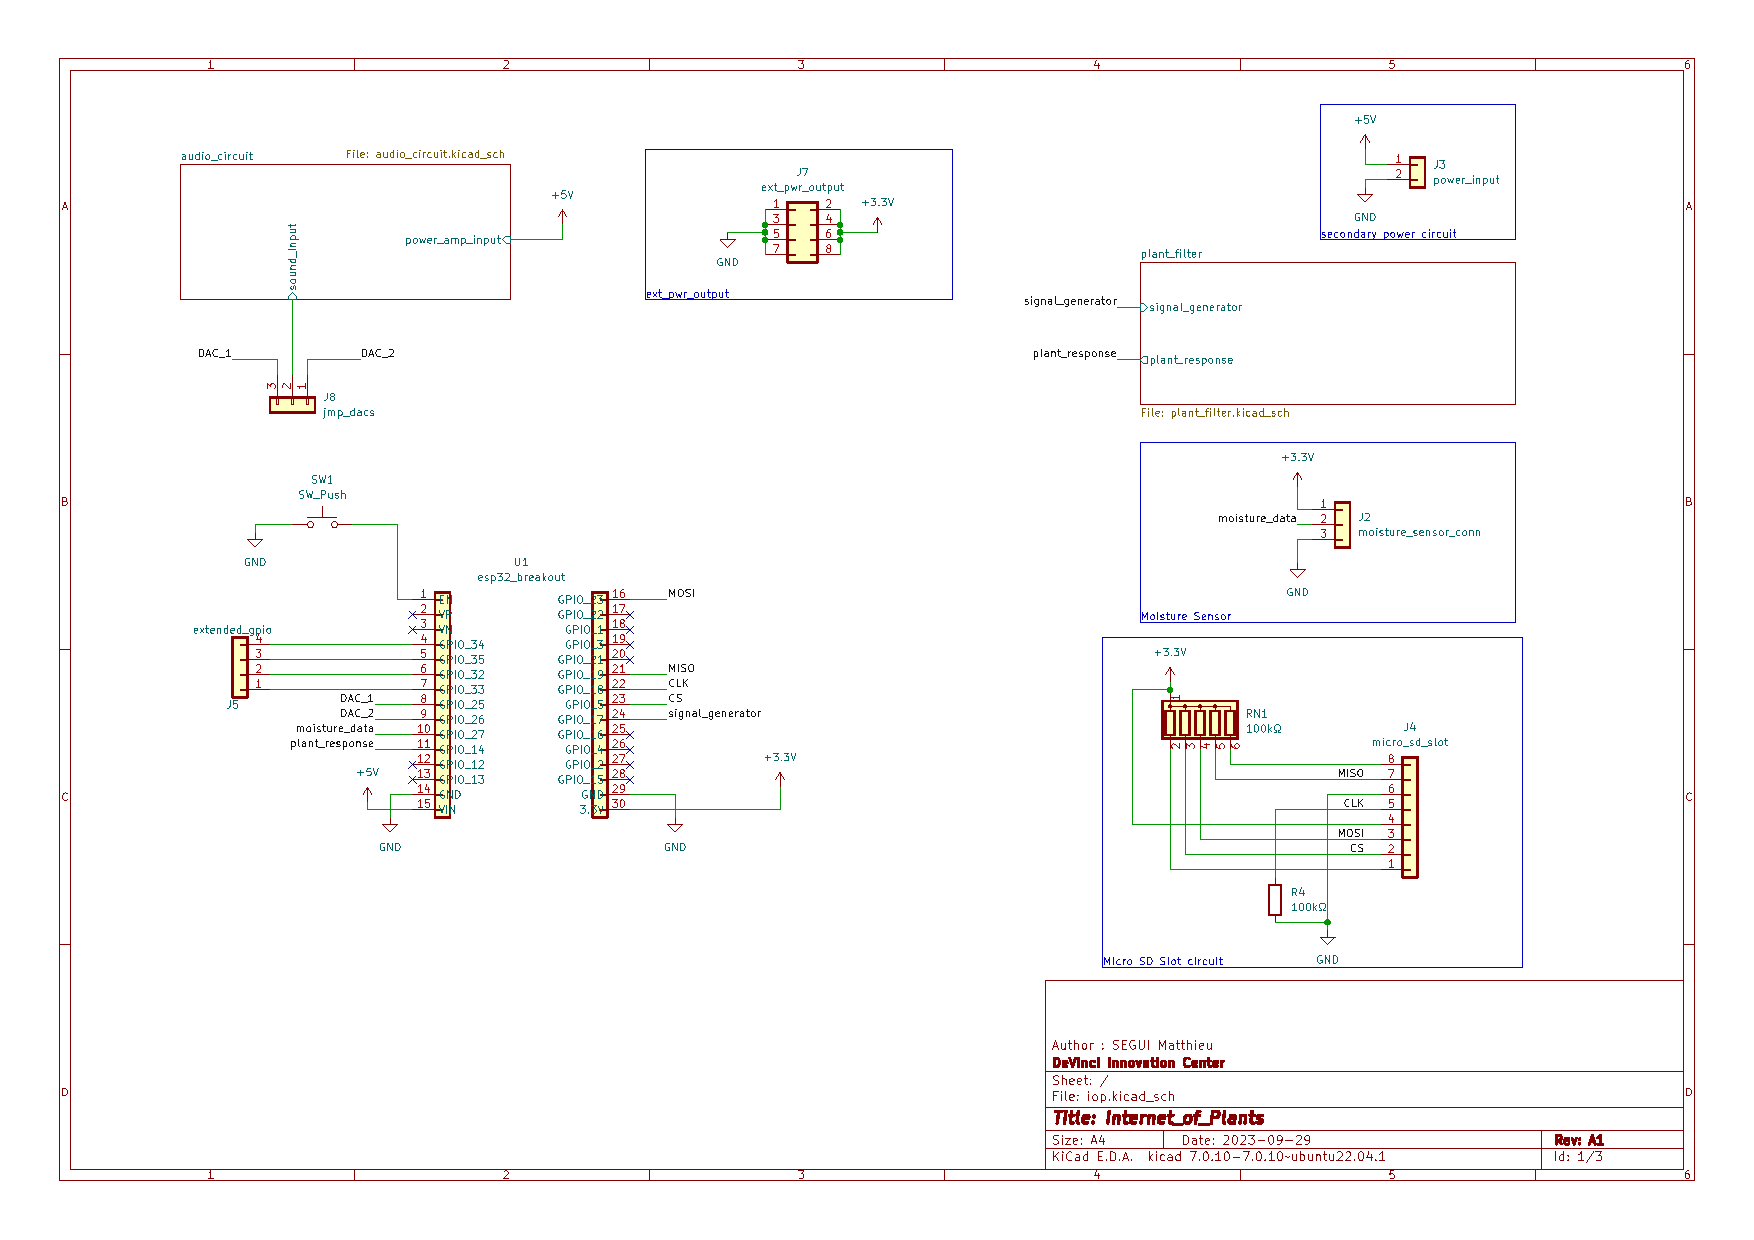
\includegraphics[width=\textwidth]{images/iop.pdf}
    \caption{The main schematic of the device. This main schematic regroups components and sub-sheets (including the audio circuit
    and the filter circuit). The main component is an ESP32 Wroom DevKit. All other components are linked to this
    microcontroller} 
    \vspace{0.1cm}
    \label{fig:iop_schematic_main}
\end{figure}

%TODO: Talk about the humidity sensor

The circuit component that allows us to read data from the plant is the electronic filter.
This filter has been designed by \textit{Jakub Nikonowicz} and \textit{Łukasz Matuszewski} 
from \textit{Politechnika Poznańska}.
Thanks to them, I adapted it for my application on my embedded device. 

\begin{figure}[h!]
    \centering
    \includegraphics[width=\textwidth]{images/iop-plant_filter.pdf}
    \caption{The electronic circuit designed to capture the interaction by analyzing the electronic
    frequency response. The circuit includes 3 resistors, 3 inductors and 3 capacitors as main components} 
    \vspace{0.1cm}
    \label{fig:iop_schematic_filter}
\end{figure}

This filter is ending by a crocodile clamp that is directly connected to the plant.

The last part of the circuit is the sound output/rendering. This circuit includes a small amplifier,
the LM386 from Texas Instruments. The rest of the circuit are components needed in order to 
induce amplification on the signal without creating to many noise and saturation.

\begin{figure}[h!]
    \centering
    \includegraphics[width=\textwidth]{images/iop-audio_circuit.pdf}
    \caption{The sound output part of the circuit that is used to render the sound. 
    This part includes a small amplifier, the LM386. The circuit also includes the components necessary
    to control and handle the amplification (reduce noise and saturation)} 
    \vspace{0.1cm}
    \label{fig:iop_schematic_audio}
\end{figure}

The PCB is built to be able to add a micro-SD slot (ref to \ref{fig:iop_schematic_main}). This micro-SD slot
allows to increase the storage of the embedded ROM. This can be used to store pre-built sounds and music 
to avoid generating a sound on-board.  


Once the schematic is done, we have to route the tracks. It exists multiple way to route PCB 
(single-sided, double-sided, multiple layers). We choose double sided, 2 layers on each side of the PCB.

\begin{figure}[h!]
    \centering
    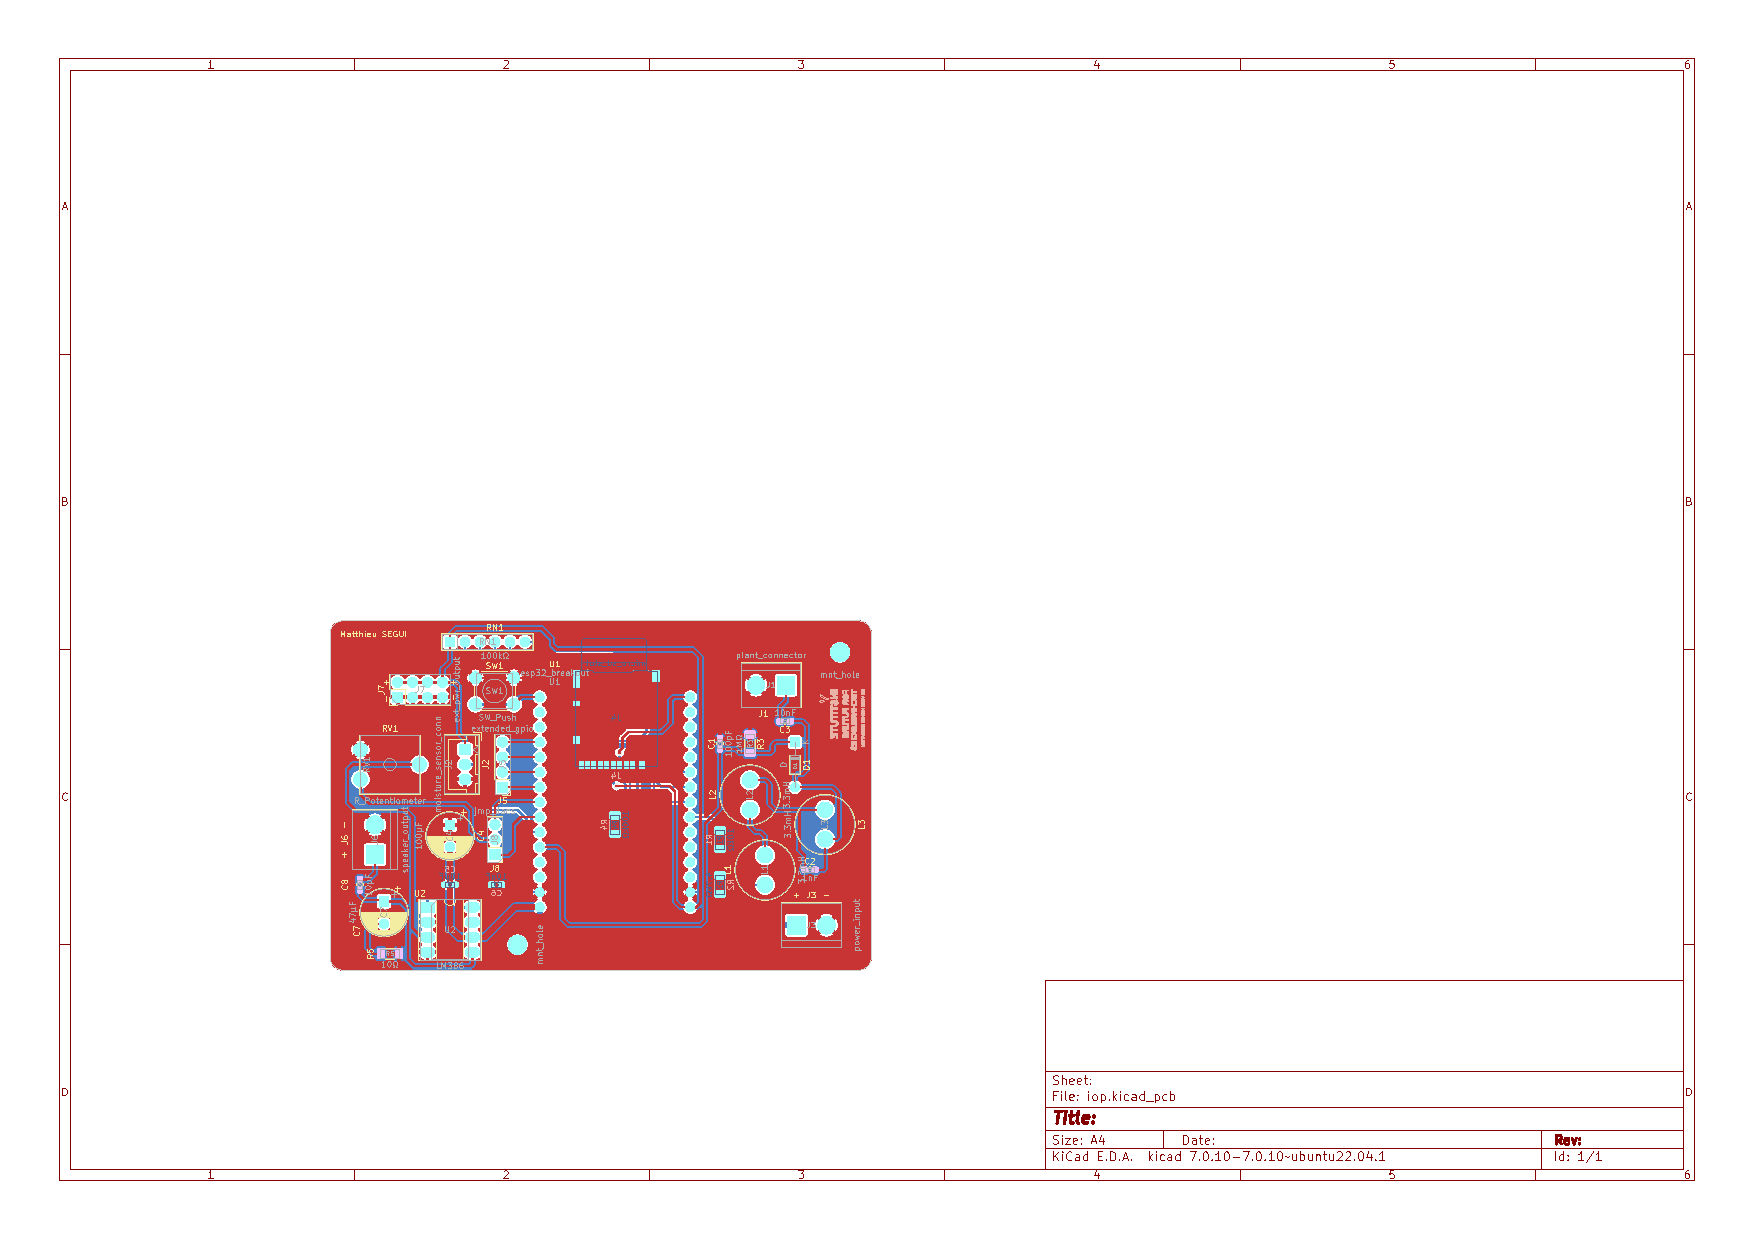
\includegraphics[width=\textwidth]{images/iop-routed_pcb.pdf}
    \caption{The routed double sided PCB.} 
    \vspace{0.1cm}
    \label{fig:iop_routed_pcb}
\end{figure}

Kicad also allows us to generated a 3D view of the future PCB. This allows us to imagine what the
PCB will look like when it will be manufactured.
\begin{figure}[h!]
    \centering
    \includegraphics[width=0.8\textwidth]{images/front_iop_3D_view_modified.png}
    \caption{Front 3D rendering of the built PCB. The rendering is done using open source software: Kicad} 
    \vspace{0.1cm}
    \label{fig:front_iop_3D_view_modified}
\end{figure}

\subsection{Human interaction}

\subsubsection{Use of the sensor/filter}

The device is able to capture the human interaction with the plant. The touch interaction is inducing changes
in the impedance, capacitance and inductance of the plant. Values are captured using the GPIO (General Port Input/Output)
14 of the ESP32 DevKit. This GPIO is able to read analog data and convert them to digital values using analog to digital
converter (ADC). The values are a floating point number between %TODO: Add the range of the values here.
Values are fluctuating depending on the interaction. 

%TODO: Add a table comparing the values depending on the interaction

The possibilities of 


\subsubsection{Sonification on the device} % FIXME: subsubsection ??

The human interaction goes through the sonification on the device. ESP32 embeds a 8-bit digital to analog converter (DAC).
The embed DAC is enough to play low quality sounds. Combined with the micro-SD card including in it, it is a media player.
Using the \textit{Arduino Audio Tools} library it is possible to read MP3, Wav and other audio format.
Taking the sensor value as an input, you can then apply a pitch shift on the data that will be rendered on the DAC.
The pitch shift is a value included between 0 and 100. We are mapping the max value of the sensor and the min value
to this range using the \textit{map()} Arduino function.

The data is sent to the DAC and rendered. \textit{Arduino Audio Tools} also includes a way to communicate data to the
DAC.

%TODO: Add oscilloscope screenshot of the sound output.

There are two DAC available on the ESP32. DAC 1 and DAC 2 respectively on GPIO25 and GPIO26. The IoP device allows
to choose between the one you want by using a removable jumper.

The output of the DAC is too low to be able to render it on a speaker. The amplification circuit allows a small 
amplification of the output. The amplifier is a basic and simple one. I added a 10k Ohms potentiometer to be able to
tweak the volume. The sound quickly reach amplifier limitations and is becoming saturated. 

The amplified output is sent to a terminal block that acts as the connection interface to the audio speaker.
The audio speaker chosen in our specific example is a 8 Ohms 3 Watts speaker. 

\begin{figure}[h!]
    \centering
    \includegraphics[width=0.8\textwidth]{images/speaker.jpg}
    \caption{8 ohms 3 Watts basic speaker used in our example.} 
    \vspace{0.1cm}
    \label{fig:speaker}
\end{figure}


\newpage
\subsubsection{User study}
\paragraph{Abstract of user study}
This study explores human-plant interaction.
This study has been conducted in order to understand what kind of interaction we have to detect in order to have the best and more natural kind of interaction with plants.
The results will be applied in the Internet of Plants (IoP) project which intends to create a fully connected bio-organ system.
The IoP is looking to reduce the gap between humans and plants by creating a symbiotic relationship between 
nature and technology. We envision a world where our daily objects are responsive.

\paragraph{Introduction}
Plants represent a full ecosystem of evolution, adaptation and communication.

In the context of the Internet of Plant (IoP) project, this study aims to extract the natural interaction between people and plants.
This experiment explores the interactions the IoP device will have to detect to create a symbiotic relation between human and plants. 
The physical touch is the starting point of a sonification process.
Sonification is “the use of non-speech audio to convey information or perceptualize data” \cite{kramer2010sonification}.
Three distinct plant species—\textit{Dypsis lutescens, Pachira glabra, and Dracaena}—are employed as subjects to extract user perceptions and interactions within this framework. 

The methodology engages students from the engineering school and two researchers.
The participants are asked to interact with the plants and imagine the sounds that could be generated by the plants.

The correlation between plant height and trunk interactions reveals environmental factors impacting human-plant dynamics.
Additionally, interactions are categorized based on intensity, spatial displacement, and duration.


\paragraph{Methodology}

\subparagraph{Participants}
The study is conducted on 22 participants. Participants are mainly composed of engineering students. The participant set includes 15 males and 7 females.
The age of participants is between 19 and 22 years old. Exception for three participants that are older than 22 years old. 




\subparagraph{The Procedure} 
We introduced the subject telling participants : 
"We're in the very near future. You are looking at plants that make music when you physically interact with them (it is not actually the case, but imagine it). Explore their capabilities."
Using this prompt, we tried not to bridle them to much but approach them to the physical interaction component.
Subsequently, participants were given time to explore the potential musical capacities of the plants at their own pace.
We conducted the study without providing any guidance during the exploration phase.
In instances where participants encountered difficulty initiating exploration, the prompt was reiterated to encourage the participants to explore.
This methodological approach was designed to capture the intuitive and natural human-plant interaction.
Also, we avoided any kind of communication or talking between 2 participants to reduce the potential bias.


\subparagraph{Materials/Tools}

To proceed and conduct this user study, we chose 3 different plants from 3 different species.


\textit{\textbf{Dracaena}}: It has long leaves and fragile perceived trunk but also flexible. The plant is 95 cm tall.

\begin{figure}[h!]
    \centering
    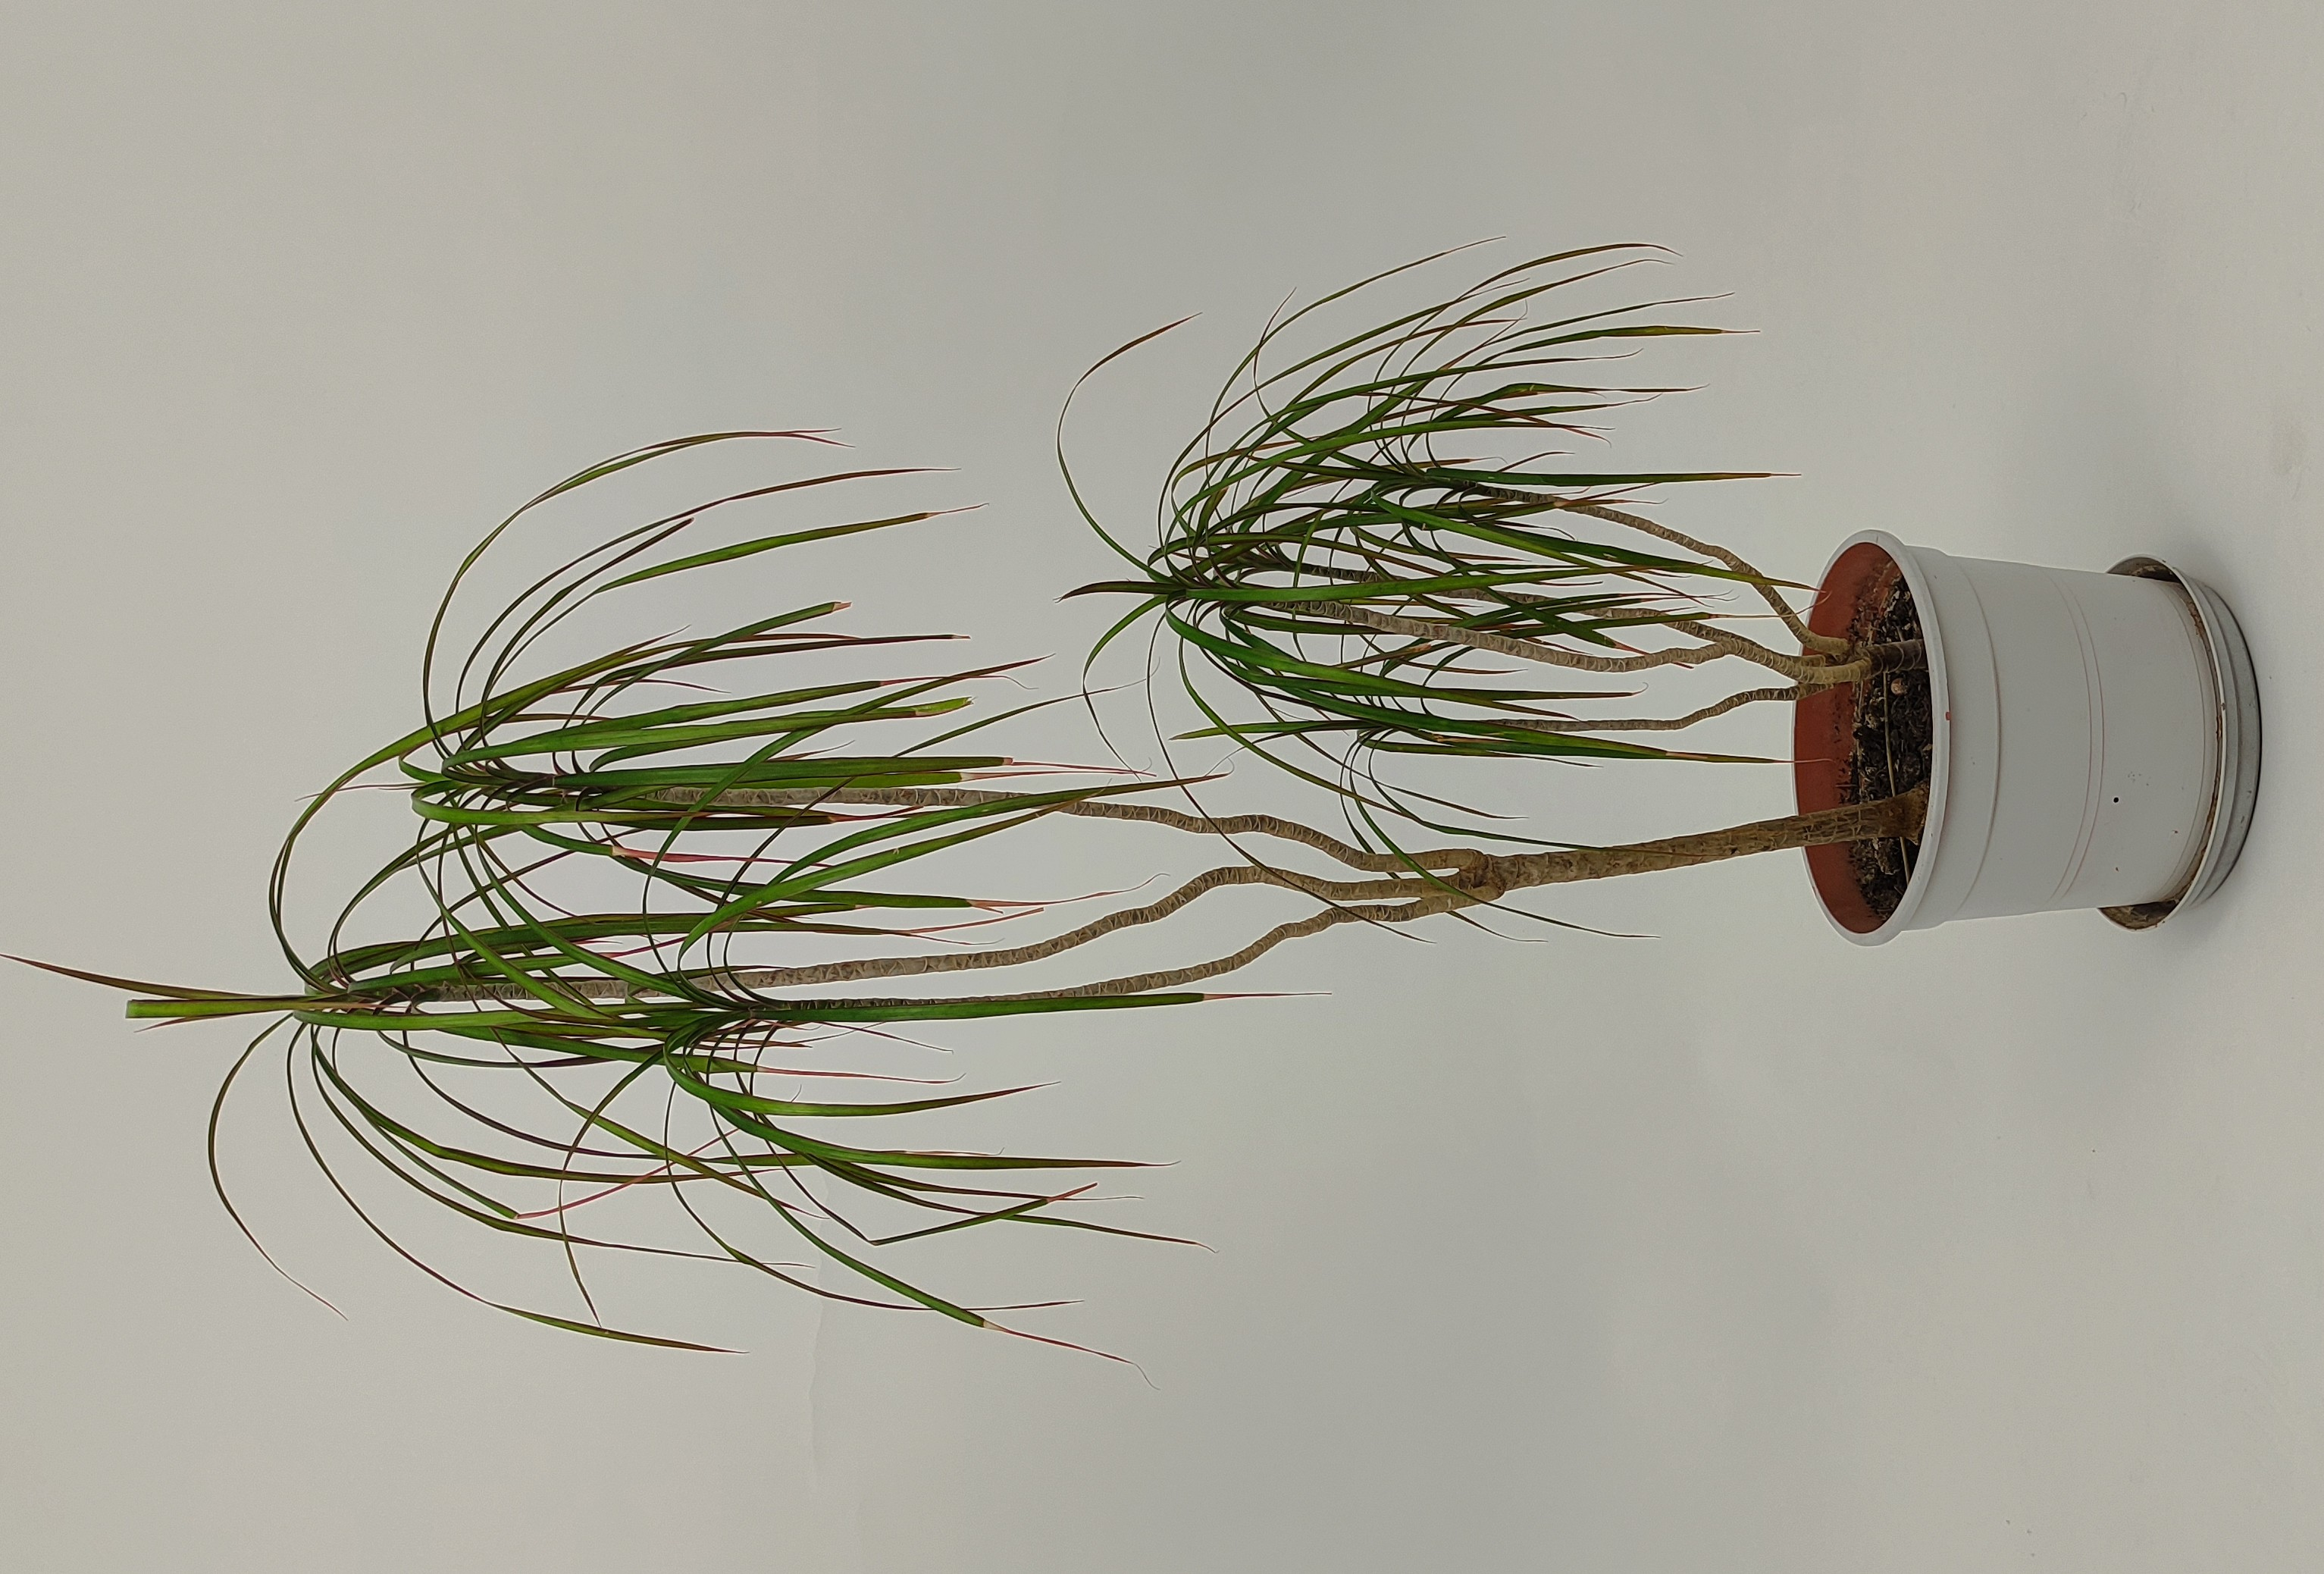
\includegraphics[width=0.8\textwidth, angle=-90]{small_plant.jpg}
    \caption{The N°1 plant is a \textit{Dracaena}.}
    
    \vspace{-0.5cm}
    \label{fig:small_plant}
    \vspace{0.2cm}
\end{figure}




\textit{\textbf{Pachira glabra}}:We chose to use this plant for its large leaves and its wide trunk.
The plant is 110 cm tall.

\begin{figure}[h!]
    \centering
    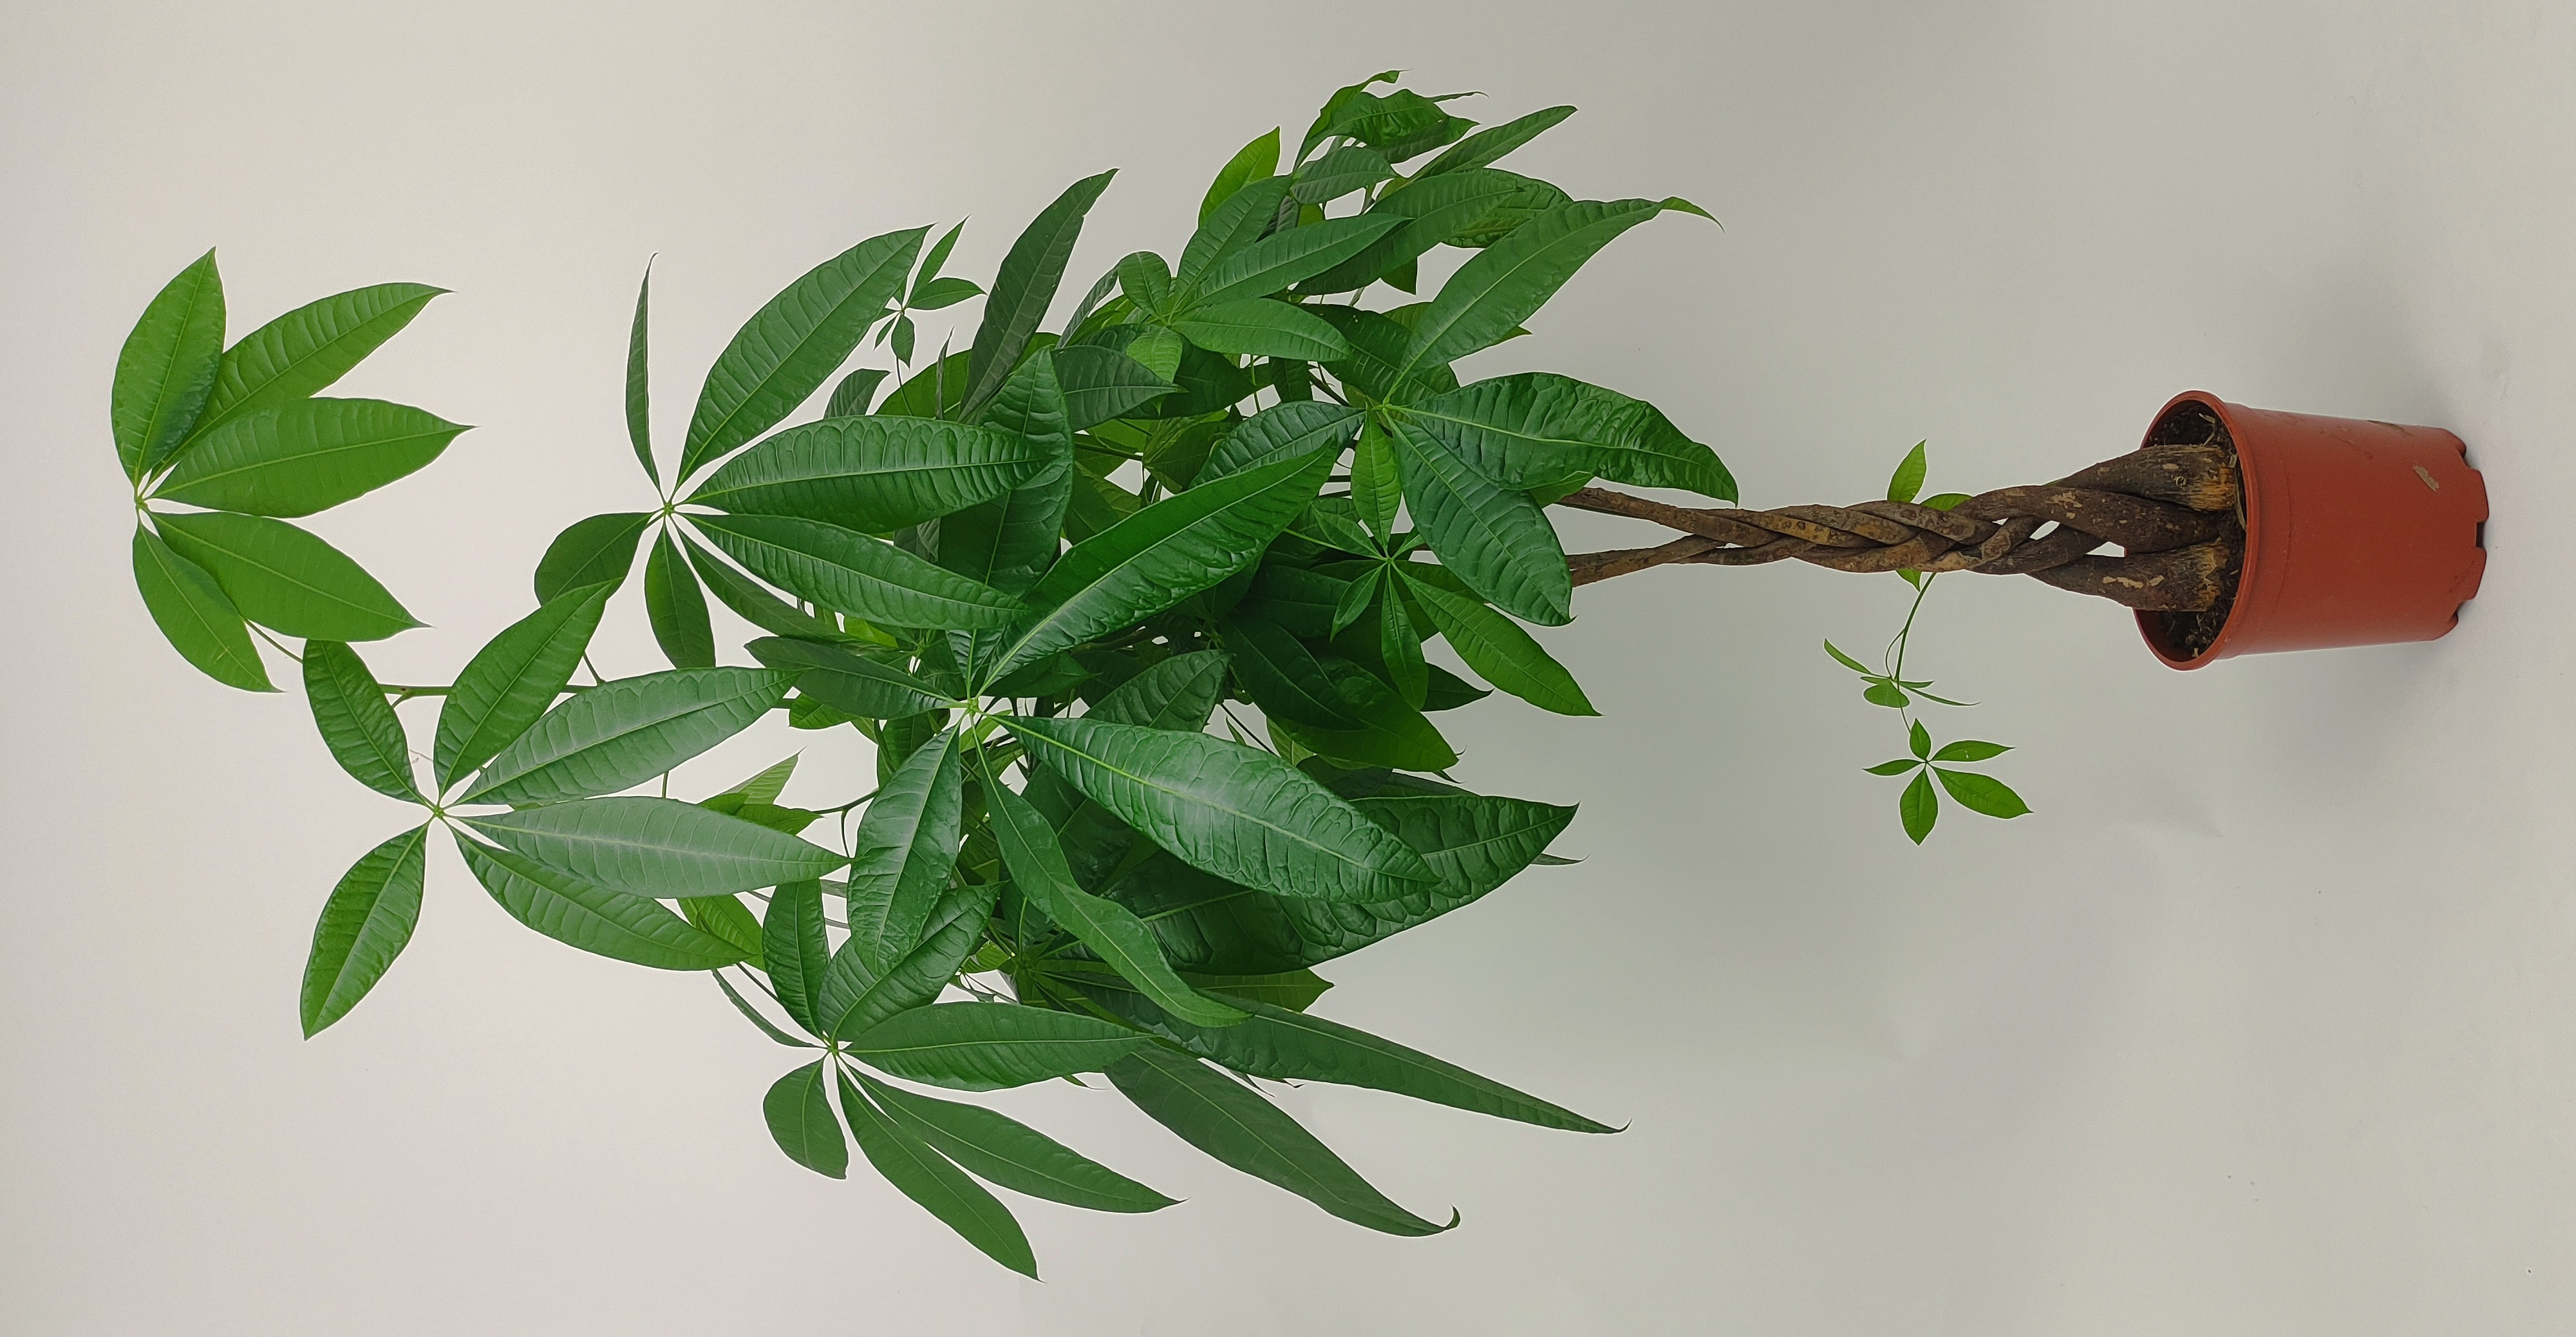
\includegraphics[width=0.8\textwidth, angle=-90]{tall_plant_cropped.jpg}
    \caption{The N°2 plant is a \textit{Pachira glabra}.}
    
    \vspace{-0.5cm}
    \label{fig:tall_plant}
    \vspace{0.2cm}
\end{figure}



\textit{\textbf{Dypsis lutescens}}: The \textit{Dypsis lutescens} is composed of many trunks and stems. On top of that, the leaves are numerous and tight. The plant is \hl{...} tall.

\begin{figure}[h!]
    \centering
    \includegraphics[width=0.8\textwidth, angle=-90]{fougere_plant.jpg}
    \caption{The N°3 plant is a \textit{Dypsis lutescens}.}
    
    \vspace{-0.5cm}
    \label{fig:fougere_plant}
    \vspace{0.2cm}
\end{figure}



\subparagraph*{The experimental space}
The experimental space featured three distinct levels of height, each corresponding to one of the three plants introduced to participants.

\begin{figure}[h]
    \centering
    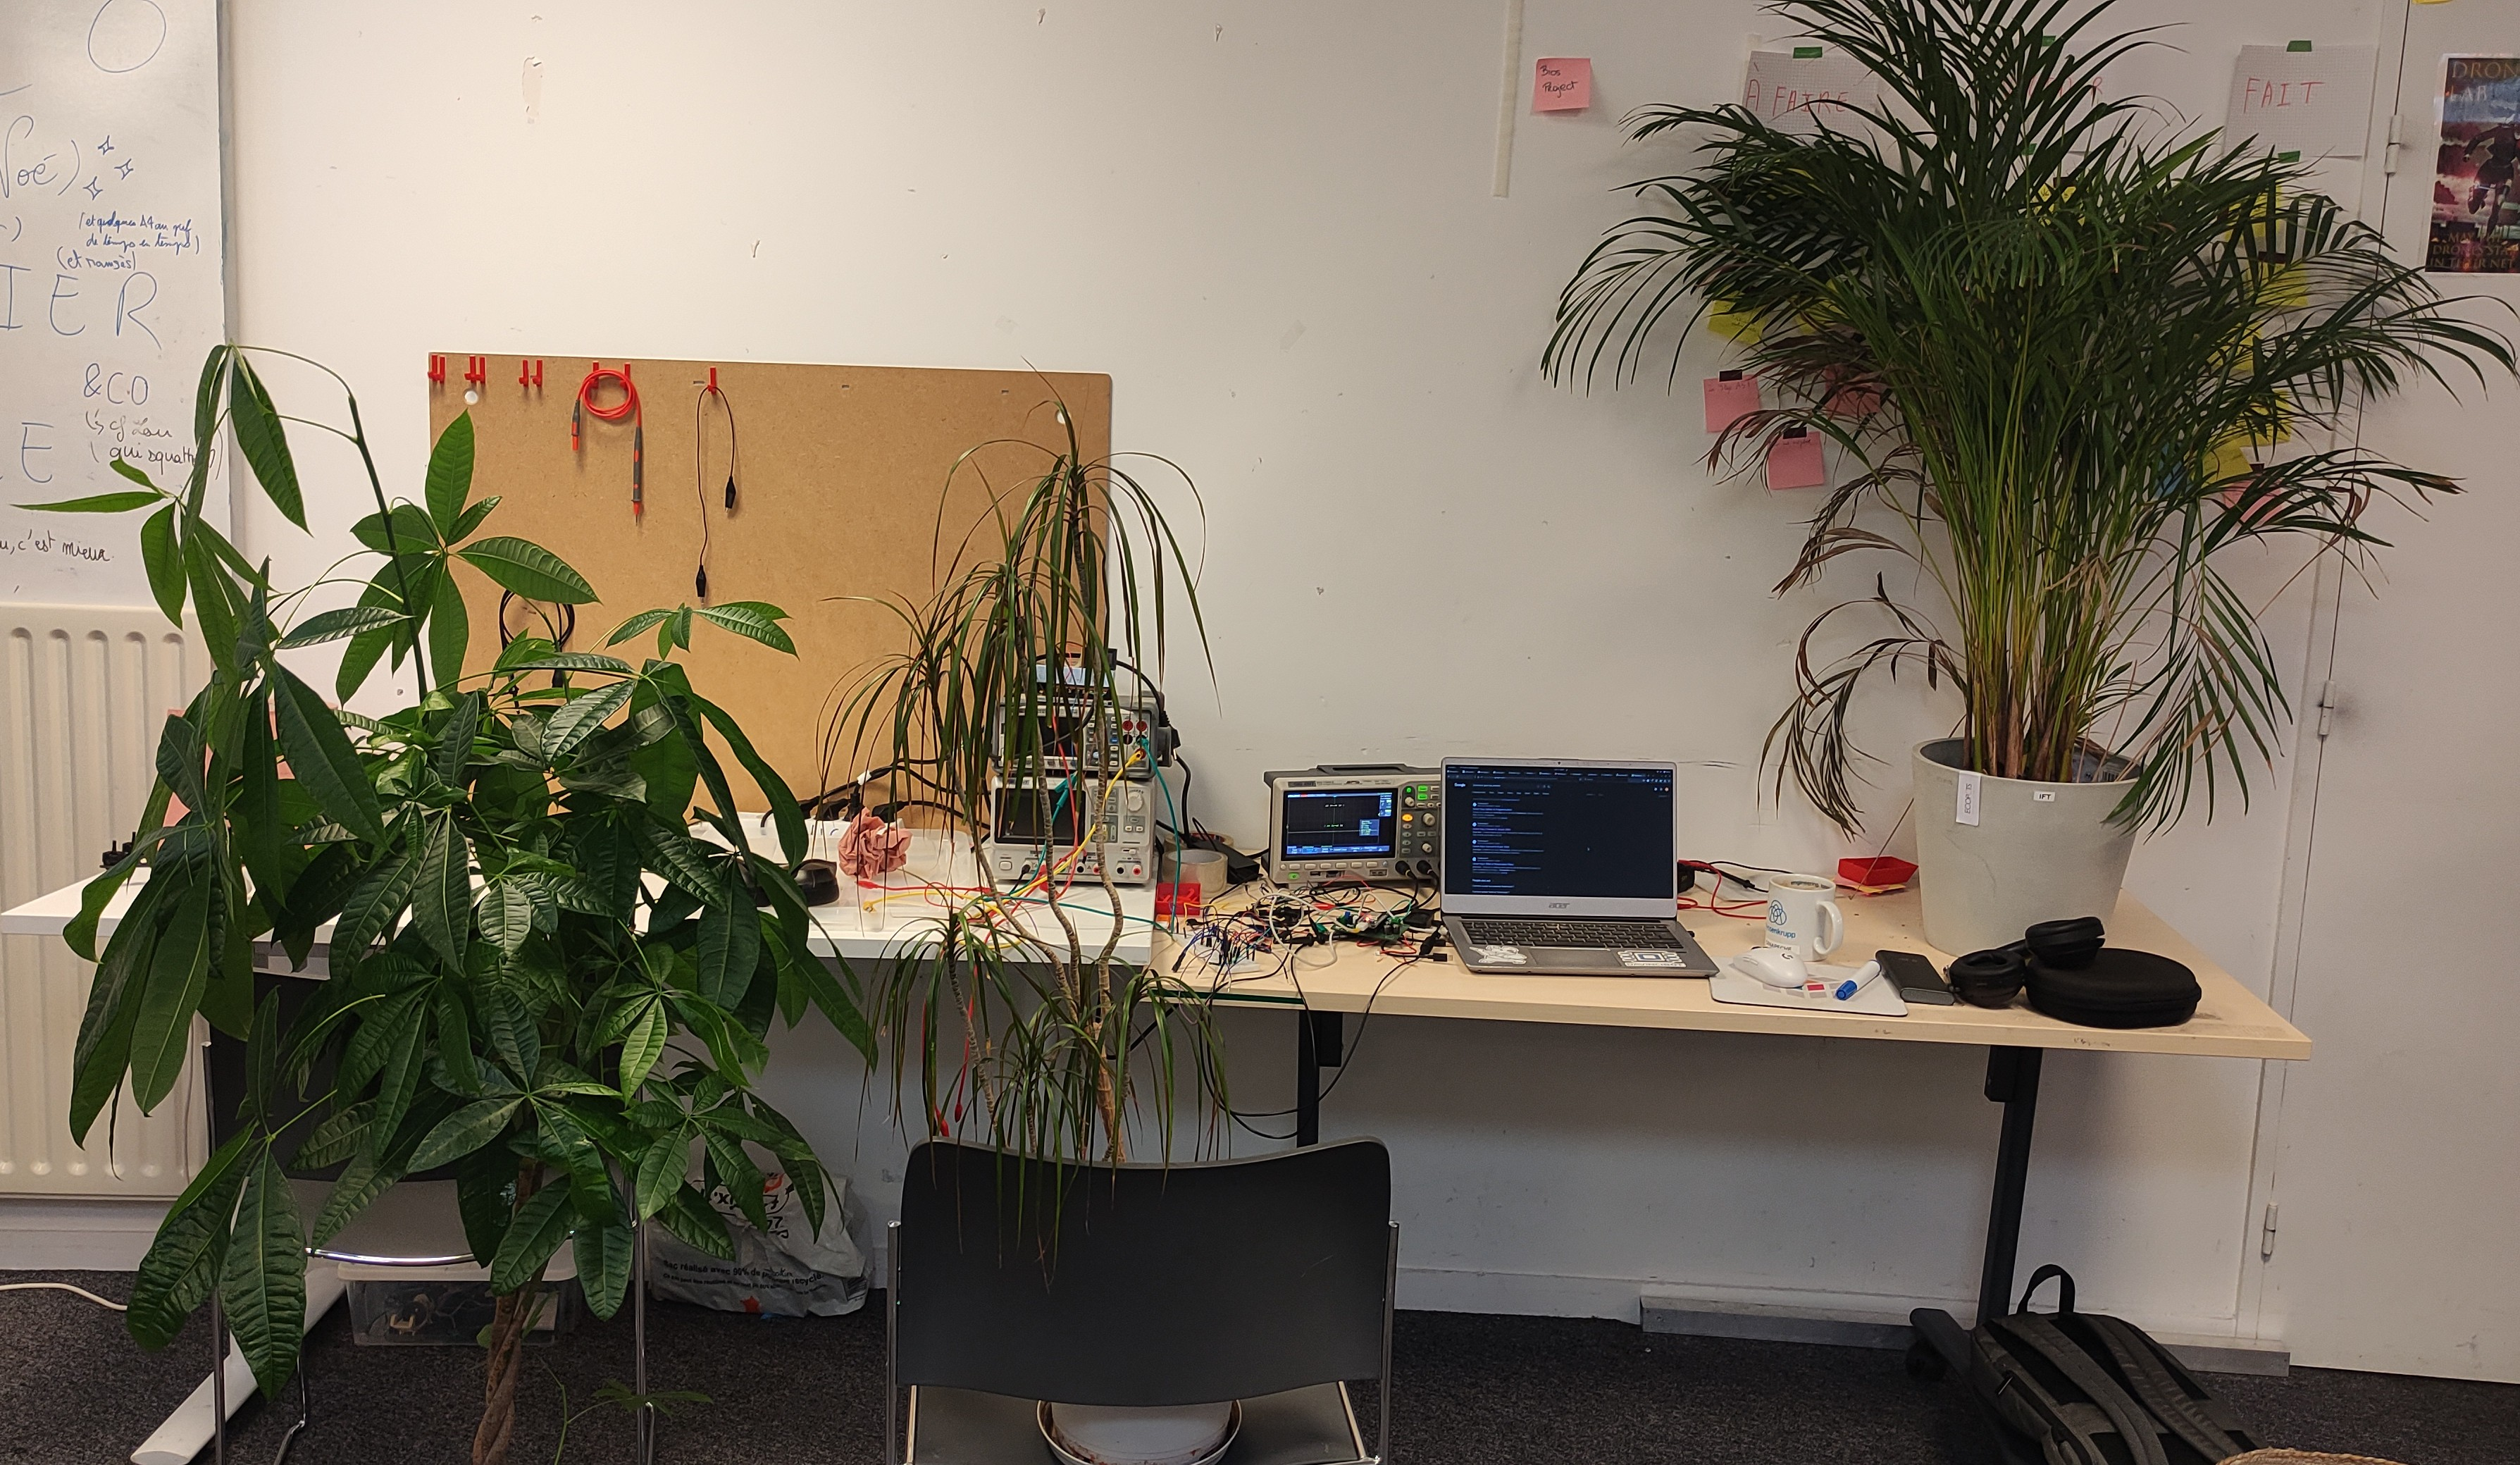
\includegraphics[width=0.8\textwidth]{setup_user_study.jpg}
    \caption{User study space setup. The setup is built from our lab space.}
    
    \vspace{-0.5cm}
    \label{fig:setup_user_study}
    \vspace{0.2cm}
\end{figure}

\paragraph{Data collection}
To capture the participant's interactions with the plants, a collaborative approach was adopted, involving two researchers to provide dual perspectives.
Throughout the exploration phase, both researchers took notes, documenting the diverse ways in which participants engaged with the three distinct plants.
The researchers explicitly specified the plant involved in the interaction in order to extract special features related to a specific plant.

The written notes retrieved descriptions of participants' actions, movements and interactions.
The dual-observer strategy tends to reduce the potential biased.

At the beginning of the experiment, the \textit{Dypsis lutescens} was on the floor, the \textit{Dracaena} was on a chair and the \textit{Pachira Glabra} was on a table.
At the middle of the experiment, we switched the \textit{Dypsis lutescens} and the \textit{Pachira Glabra} to see if the participants would interact differently with the plants.
The set-up of the experiment is shown in Figure \ref{fig:setup_user_study}. 


\paragraph{Results}

The data given by the user study allowed us to define 5 main types of interaction. Those interactions are defined by the way the user interacts with the plant. The 5 main types of interaction are :

\begin{itemize}
    \item Grasp : user uses the whole hand to grab trunk or leaves.
    \item Pinch : user uses 2 to 3 digits to grab trunk or leaves.
    \item Slide : user uses his/her hand or finger to slide on the plant whether is on a leave or on the trunk. The action is continuous.
    \item Pet : user uses his/her hand to cuddle the plant or to pass through the leaves. The user is moving his/her hand in space. She/he is not staying still or staying on a particular object.
    \item Tam Tam : user taps on the plant mainly using the whole hand.
\end{itemize}



Looking at the results, we extracted the table \ref{tab:results}.


\begin{table}[ht]
\begin{tabular}{|l|ll|l|ll|}
\hline
\multirow{2}{*}{Plant/Interaction} & \multicolumn{2}{l|}{Group 1}       & Group 2 & \multicolumn{2}{l|}{Group 3}       \\ \cline{2-6} 
                                   & \multicolumn{1}{l|}{Grasp} & Pinch & Slide   & \multicolumn{1}{l|}{Pet} & Tam Tam \\ \hline
Plant N°1                          & \multicolumn{1}{l|}{4}     & 8     & 4       & \multicolumn{1}{l|}{4}   & 2       \\ \hline
Plant N°2                          & \multicolumn{1}{l|}{9}     & 3     & 3       & \multicolumn{1}{l|}{3}   & 10      \\ \hline
Plant N°3                          & \multicolumn{1}{l|}{10}    & 1     & 5       & \multicolumn{1}{l|}{7}   & 3       \\ \hline
Total                              & \multicolumn{1}{l|}{23}    & 12    & 12      & \multicolumn{1}{l|}{14}  & 15      \\ \hline
\end{tabular}
% \caption*{Plant N°1 : Petite | Plant N°2 : Grande | Plant N°3 : Fougère}
\caption{Raw results extracted from the user study}
\label{tab:results}
\end{table}


With the extraction of the result we were able to design a bar chart.
The graph is grouping the interactions by plant. The height of the bar is the number of participants that performed the interaction.
The graph is shown in figure \ref{fig:setup_user_study}.


\begin{figure}[ht]
    \centering
    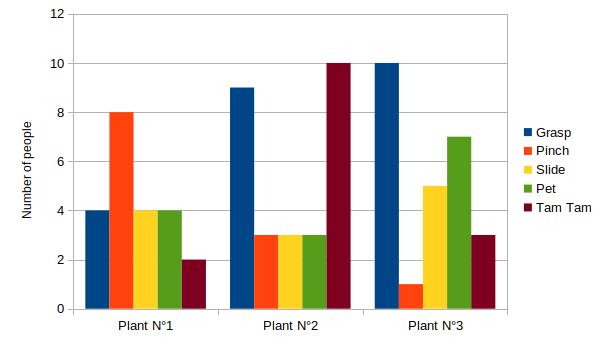
\includegraphics[width=\textwidth]{plant_interaction_chart_2.png}
    \caption{Bar chart that is extracting the main types of interaction regarding each plants.}
    
    \vspace{-0.5cm}
    \label{fig:chart_interaction}
    \vspace{0.2cm}
\end{figure}

In the end, of the 22 participants, 15 were already familiar with the project and 7 were not.

\paragraph{Discussion}
Looking at the results, the interaction were various depending on the plant. 
Thus, we can extract main interactions that are linked to the plant type. 
Looking at table \ref{tab:results}, people are more inclined to use their hands as tam tam or grasp the \textit{Pachira glabra}. 
However, for the \textit{Dracaena} users prefer to pinch the trunk or leave. 
Participants decided to grasp whether a pack of trunk or leaves when it came to \textit{Dypsis lutescens}.
This is induced by many factors including the leaves shape, the width of the trunk.


It was observed that when the plants were positioned at higher elevations on the table, individuals tended to engage more with the trunk of the plants.

Looking at table \ref{tab:results}, we decided to group interaction. This was done by grouping type of interaction depending on 3 main factors :

\begin{itemize}
    \item The intensity factor : what is the intensity of the interaction (ex : pinch is lighter than grasp)
    \item The spatial factor : what is the interaction displacement.
    \item The duration factor : what is the interaction duration (ex : tam tam is instantaneous).
\end{itemize}

The "Group 1" includes the pinch and grasp interaction. Indeed, looking at the 3 factors we defined, 
the pinch and grasp are high in intensity and long in duration but people stay still in space.
This group of interaction can be defined as \textbf{binary interaction}. The user is either grasping or not.

The "Group 2" includes the slide. The slide interaction is long in time, it moves in space but low in intensity.
This group of interaction can be defined as \textbf{continuous interaction}.


Whereas, the "Group 3" includes the pet and Tam Tam. 
These 2 interactions are really high in intensity, people usually tam tam and pet in different places but those interactions are short in time. 
This group is defined as \textbf{repetitive interaction}. The user is repeating the same action over and over again.


\begin{figure}

    \begin{minipage}{.5\linewidth}
    \centering
    \subfloat[]{
        \includegraphics[scale=.4]{group_1_int_dia.png}
        
        \label{fig:interactions:subfig:group1}
        }
    \end{minipage}%
    \begin{minipage}{.5\linewidth}
    \centering
    \subfloat[]{\label{fig:interactions:subfig:group2}\includegraphics[scale=.4]{group_2_int_dia.png}}
    \end{minipage}\par\medskip
    \centering
    \subfloat[]{\label{fig:interactions:subfig:group3}\includegraphics[scale=.4, width=0.5\textwidth]{group_3_int_dia.png}}
    
    \caption{Figure showing graphically the intensity of the 3 types of factors we defined. (a) Group 1 : pinch and grasp. (b) Group 2 : slide. (c) Group 3 : pet and tam tam.}
    \label{fig:main}
    \end{figure}


The participants we interviewed introduced a bias in the results.
They were all students from the engineering school and thus, they all had a similar background.
Some of them were already familiar with the project.

\paragraph{Conclusion}

During our study on the Internet of Plant project, we've captured insights into how people might interact with plants in a future where they make music through touch.

Our three chosen plants influenced how participants engaged with them. We observed everything from gentle petting to energetic drumming on the plants.
Interestingly, we found that when the plants were higher up, participants tended to focus more on the trunk.

By grouping interactions based on factors like intensity and duration, we gained a clearer picture of how people approached these musical plants.
It turns out that certain interactions, like grasping and pinching, were more common, while others, like sliding, had their own distinct appeal.

Regarding to the results we thought about what could be done with the defined interactions.
For instance, the sound generated from the interaction could be linked to the kind of interaction.
People doing Tam Tam on the plant will expect a drum sound. Whereas, people performing a slide will expect a sound closer to a continuous organ sound.
The possibilities are endless and the only restrictions are the capabilities of the device capturing the interaction. 
\subsection{Evaluation ?}
% 1. Technical Performance Testing

%     Accuracy of Plant Signal Capture: Measure how effectively the electronic filter captures changes in the plant's impedance, capacitance, and inductance when touched. This can be done by comparing sensor output data with known interactions to determine precision.
%     System Responsiveness: Test the responsiveness of the ESP32 microcontroller to human interaction with the plant. Evaluate the delay (latency) between the interaction and the corresponding sensor reading.
%     Signal Integrity: Assess the quality of the signals captured, ensuring that they are free from noise and distortion. Testing under varying environmental conditions (e.g., humidity, temperature) could be useful to ensure robustness.

% 2. User Study (Usability Testing)

%     Human Interaction Evaluation: Conduct controlled experiments to observe how users interact with different plant species, as detailed in the thesis. Participants can be asked to engage with the plants intuitively, and the interactions can be categorized as in the existing user study (e.g., pinch, grasp, slide). This helps evaluate the naturalness and intuitiveness of the plant as an interface.
%     User Satisfaction: Gather qualitative feedback from users on their experience interacting with the plants and the system's ability to translate their touch into meaningful sound. Surveys or interviews can help measure how engaging and satisfying the interaction feels.
%     Cross-species Comparison: Extend the existing user study to a wider variety of plants to ensure the system's adaptability across different plant types.

% 3. Sonification Quality

%     Audio Feedback Appropriateness: Evaluate the correlation between plant interaction and sound output. Test whether users perceive the generated sound as natural and whether different interactions (e.g., light touch vs. strong grasp) produce distinguishable auditory outputs. This could be assessed with a mixed-methods approach (e.g., user ratings and auditory analysis).
%     Sound Quality: Measure the quality of the sound generated by the embedded DAC and amplifier in terms of clarity, volume, and distortion.

% 4. System Stability and Scalability

%     Stress Testing: Test how the system behaves under continuous use and under varying loads (e.g., multiple touches in rapid succession). This will assess the system’s durability and resistance to breakdowns.
%     Scalability: Investigate whether the system can handle an increased number of sensor connections (additional plants) without performance degradation. This can be done by adding more plants and monitoring the system's response.

\subsection{Discussion}

The final product is an embedded device that include signal filtering, wireless communication and embedded sonification.


% To improve the device, the PCB could be reduced in size using a surface mounted device (SMD) ESP32 instead of a DevKit.
% I already started to work on a new version of the device. This version is only designed on Kicad and not prototyped.
% The rest of circuit is similar. 

%TODO: Add a schematic of the new PCB


A better audio amplifier could be explored in order to reduce the distortion of the sound.
Adding an external digital to analog converter is also a possibility in order to upgrade the output. However,
this possibility adds new components that will increase the size. Exploring the I2S protocol opens better output.
The I2S protocol is a protocol  %TODO: Talk quickly about I2S protocol


\subsection{Conclusion}

In conclusion, the standalone electronic system demonstrates significant potential in transforming natural plants into interactive bio-sensors, using the capabilities of a powerful microcontroller like the ESP32. The system's ability to capture plant responses to human touch and translate them into digital data is made possible by its efficient electronic interface. This architecture enables real-time interaction and offers new approach to human-plant interaction. This is also driving research into the use of plants' natural capacities as sensors. However, despite the microcontroller's strengths, the system still has notable limitations.

One major challenge lies in the sonification process, where the system struggles with producing high-quality, nuanced sound outputs due to the basic 8-bit DAC and limited audio amplification. Additionally, the data processing capabilities of the standalone device are limited, restricting the complexity of interactions it can detect and interpret. The sensor accuracy also has room for improvement, particularly in capturing fine-grained variations in plant interaction, which could taint the overall user experience and reduce the immersion.

To overcome these standalone limitations, a more sophisticated architecture is required. By connecting multiple devices in a distributed system, the Internet of Plants approach can enhance the processing power, improve sonification through external software, and allow for more complex data analysis. It could unlock the  full potential of plant-based sensors. The next section will explore how this expanded network can significantly enhance both the system's capabilities and user experience.
\section{Internet of Plants}

\subsection{Overview}

The Internet of Plants, also called IoP, is a concept that aims to interconnect the plant device previously built.
This in order to empower the device capabilities and to provide a better user experience.
This project includes:
\begin{itemize}
    \item A better sound quality by using professional sonification software
    \item The ability to create a full artistic experience by creating a distributed instrument
    \item Refining the interaction with the plant by using more complex data analyses
\end{itemize}



\subsection{Communication}

On the communication side, we benchmarked several communication protocol including internet protocol,
Bluetooth, Bluetooth Low Energy and Zigbee (ref to table \ref{tab:protocol_comparison}).

\begin{table}[]
    \begin{tabular}{|l|l|l|l|l|}
        \hline
        Protocol                            & IP   & Bluetooth & BLE   & Zigbee \\ \hline
        Handle multiple connections         & Yes  & No        & No    & Yes    \\
        Requires additional hardware        & No   & No        & No    & Yes    \\
        Subject to interference             & Yes  & Few       & Few   & Yes    \\
        Energy efficiency (using a battery) & Days & Months    & Years & Years  \\ \hline
    \end{tabular}
    \caption{Comparison between different communication protocol to find the one that will suits our needs.}
    \label{tab:protocol_comparison}
\end{table}

The IP protocol (whether it is on WiFi or Ethernet) has been chosen for this application for several reasons:

\begin{itemize}
    \item \textbf{High bandwidth}: It supports the transmission of large amounts of data quickly and efficiently, which is essential for real-time interactions in the system.
    \item \textbf{Widespread availability}: WiFi and Ethernet are commonly available in most exhibition spaces, ensuring easy deployment in a variety of environments.
    \item \textbf{Multi-device connectivity}: The protocol allows the connection of multiple devices simultaneously, which is crucial for building a distributed system where many plants can interact with the server.
    \item \textbf{Compatibility}: Ethernet is already available on the server, and WiFi is built into the ESP32, eliminating the need for additional hardware.
\end{itemize}

The communication system is based on WiFi technology, leveraging the ESP32's built-in wireless capabilities. Both the server and the ESP32 devices are connected to the same local network. Data is transmitted from the ESP32 to the server using the IP protocol via a TCP (Transmission Control Protocol) socket. Each ESP32 opens a dedicated TCP socket to the server, and the server is capable of handling multiple sockets simultaneously—one for each connected device. The server is connected to the local network via an Ethernet cable, providing a stable, high-speed connection for data processing and sonification (ref figure \ref{fig:network_architecture}).

\begin{figure}[h]
    \centering
    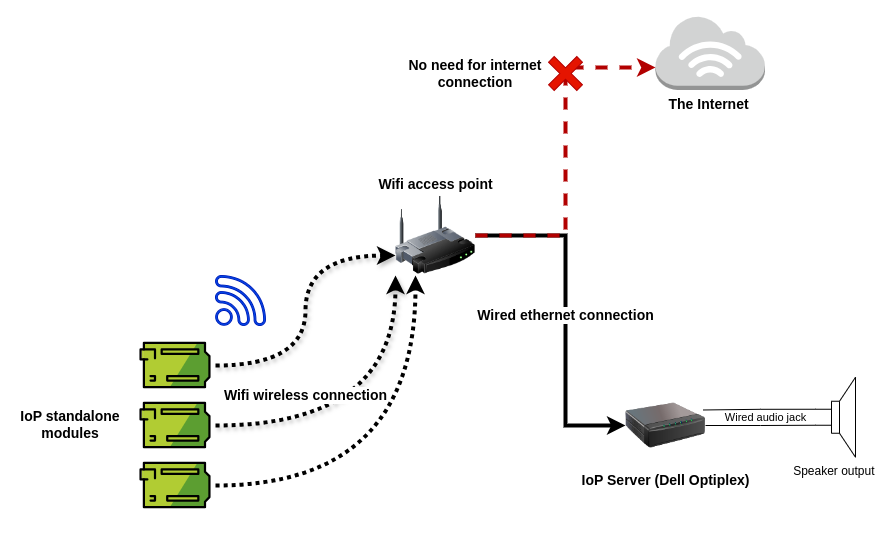
\includegraphics[width=\textwidth]{network_architecture.png}
    \caption{Schematic of the network architecture of the Internet of Plants project. The standalone modules are connected to the server using WiFi. The server is connected via Ethernet cable to the local access point. The server is also connected to a jack speaker working as output.}
    \vspace{0.1cm}
    \label{fig:network_architecture}
\end{figure}

However, a potential drawback of using IP networks is that they can become overcrowded, especially in environments with high network traffic, which may lead to packet loss or truncated data frames. To mitigate these issues, a start ("#") and stop (";\\n") character is embedded in the data transmission protocol. This structure helps the server recognize the beginning and end of each message, allowing it to discard incomplete or corrupted frames and process only complete, intact data. This approach minimizes the impact of network congestion by ensuring that even if a frame is truncated or lost, the server can still recover and process the next full message without error.

Additionally, this strategy helps maintain a balance within the CAP theorem (Consistency, Availability, and Partition tolerance). While it is impossible to achieve all three properties perfectly in a distributed system, the chosen protocol structure ensures data consistency by filtering out incomplete messages, availability by maintaining active connections across multiple devices, and some degree of partition tolerance in the event of temporary network failures. This balance is critical for ensuring reliable data transmission and processing in the Internet of Plants system.





\subsection{Server}

The server is a small fanless computer (Dell Optiplex) running Lubuntu. Lubuntu is a lighter version of Ubuntu that includes LXQt as desktop environnement. The choice of a distribution with graphical interface is induced by the use of \textit{Pure Data} as sonification software. However, the server can be run without graphical interface when on production mode. The choice of the light desktop environment is induced by the fact that the server is a low resources computer. The server only include 1 GB of RAM which is a limitation. The server is connected to the local network using an Ethernet cable. The server is also connected to a jack speaker (ref figure \ref{fig:network_architecture}).




%TODO: Add a picture of the  real setup

\textit{Pure Data} (PD) is an open-source visual programming language designed primarily for creating interactive multimedia applications, particularly in the fields of audio, video, and graphical processing.
\textit{Pure Data} is part of a family of patcher programming languages, which also includes Max/MSP.
Unlike traditional text-based programming, PD uses a graphical interface where users connect
"objects" with virtual patch cables to create complex data flows and signal processing chains.
Its modular design allows for real-time manipulation of sound and graphics, making it a powerful
tool for artists, musicians, and researchers interested in exploring experimental media.

\textit{Pure Data} requires, in a development environnement, a graphical interface to test and debug.
The \textit{Pure Data} patch receive the data through a TCP socket. The data is processed through several
operations. Then, if a threshold is passed, an interaction happened and the music is triggered.
The music is outputted through the item \textit{DAC} which means Digital to Analog Converter.
The digital input from \textit{Pure Data} is converted to a sound that speakers can output.

\begin{figure}[h]
    \centering
    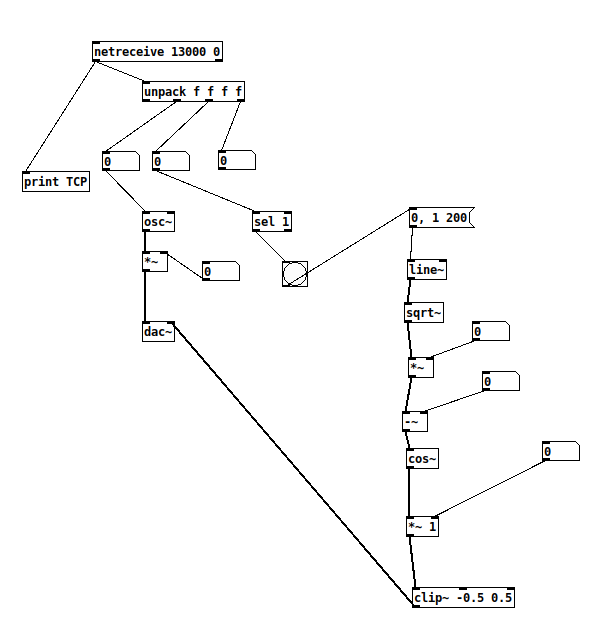
\includegraphics[width=\textwidth]{pure_data_patch.png}
    \caption{Basic \textit{Pure Data} patch that is used for sonification of the data
        of the plant. In case of an art exhibition, the \textit{Pure Data} patch can be upgraded to meet the
        artist needs}
    \vspace{0.1cm}
    \label{fig:pure_data_patch}
\end{figure}


\textit{Pure Data} is a sonification software that require data as input. In order to get and process the data, we designed a Python based software. %FIXME: microservices
The software is object oriented. The standalone IoP modules connect using WiFi to the receiver module
of the software. The connection is made using TCP socket from the ESP32 to the server.
The main module of the software then creates software abstraction of the standalone module.
The abstraction module is processing and storing all the processed data.
The main module then send the processed data to \textit{Pure Data} patch using also local TCP socket.

\begin{figure}[h]
    \centering
    \includegraphics[width=\textwidth]{iop_architecture.png}
    \caption{Architecture diagram of Internet of Plants project centered on server-side.}
    \vspace{0.1cm}
    \label{fig:server_architecture}
\end{figure}


\subsection{Deployment} %and application}

The server software is easily deployable. The software includes a shell script to deploy the server service (ref figure \ref{fig:install_script_logic}).
Indeed, the server relies on a \textit{systemd} linux service. \textit{Systemd} \cite{Both2020} is a Linux software that manage application that runs \textit{daemons} or services.
\textit{Daemons} are pieces of software that run in background of the operating
system. They are mainly started at the during the boot of the operating system.

% \begin{figure}[h!]
%     \centering
%     \includegraphics[width=0.8\textwidth]{install_script_logic.png}
%     \caption{Logic of the installation script. The script install the Python dependencies, fill in the templated service file, install the service and enable it.}
%     \vspace{0.1cm}
%     \label{fig:install_script_logic}
% \end{figure}

The server is deployed using systemd service to allow the software to start with the operating system.
It waits for the network interfaces to be up and running and opens the socket.
The installation tool install Python dependencies, fill in the templated service file,
install the service and enable it. The server is able to receive data from IoP standalone
modules and use \textit{Pure Data} software for sonification. The last step is to connect
a jack speaker to the jack builtin output.

On the IoP standalone module side, it requires a software that is able to upload
firmware to an ESP32 MCU. I recommend using PlatformIO which is an open source
embedded software development platform. The firmware is developed using this platform.
The source code is written in C++ using the Arduino framework. You flash the firmware
to the chip after setting up the WiFi credentials.
The module sends all the retrieved data to the server.

\subsubsection{Distributed instruments}

The Internet of Plants (IoP) architecture enables the creation of a distributed instrument, where multiple IoP standalone modules can be deployed across different plants to form an interconnected musical system. Each module, linked to the server via WiFi, sends data collected from plant interactions, which the server then processes. By assigning unique IDs to each module, the server can differentiate between the various plants, allowing for distinct musical outputs based on the origin of the data.

The system sends this data to \textit{Pure Data} (PD), an open-source visual programming language for multimedia applications, where sound parameters such as pitch, tone, and rhythm can be finely controlled. This setup allows for highly customizable soundscapes, where each plant generates unique sounds based on user interaction, creating a rich, immersive musical experience. The distributed instrument thus transforms the interaction with plants into a collaborative musical performance, opening up new possibilities for art installations and interactive environments.

\subsection{Results}

\subsubsection{Evaluation}

The Internet of Plants (IoP) system was evaluated based on its ability to handle multiple connections and receive data from standalone modules. The system was tested with one and two standalone modules connected simultaneously to the server, sending data packets at regular intervals. The server successfully received data from all connected devices, demonstrating its capability to handle multiple connections and process data from each module independently. The results are summarized in table \ref{tab:network_results}.
The network was not really crowded. The network tested was in a residential area with 5 devices connected to the access point.

\begin{table}[h!]
    \begin{tabular}{|l|l|l|}
        \hline
        \begin{tabular}[c]{@{}l@{}}Number of \\ simultaneously connected \\ standalone devices\end{tabular} & \begin{tabular}[c]{@{}l@{}}Number of \\ data packets \\ sent from \\ standalone modules\end{tabular} & \begin{tabular}[c]{@{}l@{}}Average number\\ of data \\ packet received \\ (on 20 runs)\end{tabular} \\ \hline
        1 standalone module                                                                                 & 100 packets                                                                                          & 99.20 packets                                                                                       \\ \hline
        2 standalone modules                                                                                & \begin{tabular}[c]{@{}l@{}}100 packets\\ (from each device)\end{tabular}                             & 99.625 packets                                                                                      \\ \hline
    \end{tabular}
    \caption{Number of data packets sent from standalone module vs number of data packets received by the server. The server is able to handle multiple connections and receive data from all connected devices. We repeated the operations 20 times to get an average.}
    \label{tab:network_results}
\end{table}




%TODO: Create a Table that regroup frame dropped vs frame received
%TODO: Create a table 

\subsubsection{Art exhibition}

To push further the distributed instrument, it is possible to build an entire
musical experience for an art exhibition.
The immersive experience can take place as a fully connected forest. The music would vary
depending on the touch interaction that people have with the plants.

\begin{figure}[h!]
    \centering
    \includegraphics[width=\textwidth]{art_exhibition.pdf}
    \caption{Schematic of the IoP art exhibition. The music varies depending on the
        interaction that people have with the installation. People are immersed into the full
        musical and sonification experience.}
    \vspace{0.1cm}
    \label{fig:art_exhibition}
\end{figure}

This exhibition could allow people to rethink the way the see and interact with plants.
Plants are not seen anymore as decoration object but as a living being.
The living being is here highlighted by the fact that plants can now express their state.
The humidity level, the light intensity and other state signs are modifying the plant
reaction.


Musicians can also work in pair with plants to create songs using music from the plants.
The music coming from the plant is fully configurable with the sonification software.


\subsubsection{Final product, limitations and future work}

Final product is a software that allows the connection between multiple standalone IoP modules and a sonification software, \textit{Pure Data}. The software handle multiple connection and apply a filtering and cleaning on the data
retrieved. The data is then sent to \textit{Pure Data} for sonification.

As a demo and in order to do a photo shooting, we built up a system using the standalone module, connected through wire (ref figure \ref{fig:server_module_demo}). We used the serial communication in this demo because we did not have wireless communication usable at the shooting site. The computer is showing a visualization from the incoming data. This is a waterwall like visualization (ref figure \ref{fig:extracted_frame_demo}). The data is processed and displayed on the computer screen. The data is normalized on the y-axis. The x-axis is the sweep frequency. The graph signal at the bottom is the real-time signal. The computer is also producing the sound using \textit{Pure Data} software.

\begin{figure}[h!]
    \centering
    \includegraphics[width=0.8\textwidth]{server_module_demo.jpg}
    \caption{Server-module demo. In this specific use case, the module is connected by wire to a computer. Otherwise, the module is usable wirelessly.The computer is acting as a server. On this version of the demo, the screen is displaying a figure that is evolving depending on the touch interaction. The computer, acting as the server, is producing the sound using \textit{Pure Data} software.}
    \vspace{0.1cm}
    \label{fig:server_module_demo}
\end{figure}

\begin{figure}[h!]
    \centering
    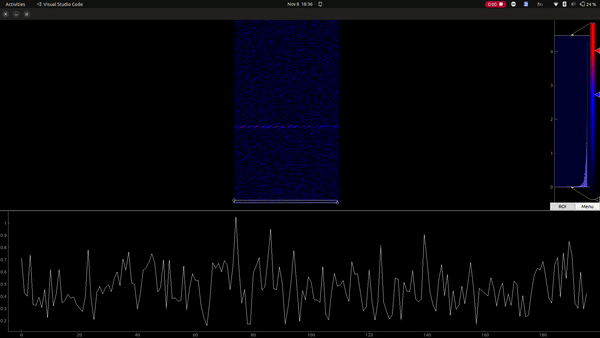
\includegraphics[width=\textwidth]{extracted_frame_demo.png}
    \caption{Waterfall like visualization of the data extracted from the standalone module. The data is processed and displayed on the computer screen. The data is normalized on the y-axis. The x-axis is the sweep frequency. The graph signal at the bottom is the real-time signal.}
    \vspace{0.1cm}
    \label{fig:extracted_frame_demo}
\end{figure}

The Internet of Plants system faces several limitations in its current implementation, particularly in the areas of communication and data reliability. One major challenge is the use of WiFi as the primary communication protocol. In environments with high network traffic, WiFi can become overcrowded, leading to dropped frames and inconsistent data transmission. This congestion affects the real-time interaction between plants and the sonification process.

Another limitation is the potential for frame loss during data transmission. Although the system incorporates start and stop tags to verify the completeness of data frames, this method is not sufficient to prevent the loss of frames in overloaded networks. The absence of a more advanced error-handling mechanism results in incomplete or corrupted data, which reduces the accuracy of the system.

Furthermore, there is limited fault tolerance in the current communication setup. The system lacks mechanisms to ensure consistent data flow or recovery from network failures, which can disrupt the continuous interaction between the plants and the server.

Lastly, there is inadequate monitoring of the distributed network. The system does not provide real-time feedback on the health of the network or the individual plant sensors, making it difficult to detect and address failures quickly.

\subsection{Conclusion}

In conclusion, the Internet of Plants (IoP) is a revolutionary application of IoT principles to plant systems, enabling more sophisticated interaction between humans and plants. By leveraging distributed systems, sensors, and sonification software, the IoP creates immersive environments where plants can become interactive instruments, generating real-time musical responses based on human touch. This innovation extends beyond artistic installations, providing new opportunities in agriculture, environmental monitoring, and human-computer interaction. However, limitations such as network congestion, sensor accuracy, and audio quality need further work to fully unlock the potential of plant-based sensor networks.



\section{Conclusion}
\vspace*{\fill}

\section*{Acknowledgements}

I would like to express my heartfelt gratitude to the three principal investigators who have guided me over the past three years. My deepest thanks go to Marc Teyssier for his invaluable support and mentorship during my UROP year, as well as to Clément Duhart and Xiao Xiao for their guidance and assistance throughout these two years of my master’s program.

I am also deeply grateful to my classmates and friends for making these two years unforgettable. A special thanks to Hugo Devoille and Paul Even, as well as to Noé Guennoun, Nicolas Leboucher, Yohann Cossez, Marc-Adrien, and many others who have been part of this journey.

Lastly, I would like to thank my professors and researchers, including Yliess, Grégor, Thomas Juldo, Paul-Peter, and Madalina, for their unwavering support and the time they dedicated to teaching us. Their efforts have equipped us with the comprehensive knowledge and skills in engineering and research, preparing us to face future challenges with confidence.
\vspace*{\fill}





%----------------------------------------------------------------------------------------

\backmatter % Denotes the end of the main document content
\setchapterstyle{plain} % Output plain chapters from this point onwards

%----------------------------------------------------------------------------------------
%	BIBLIOGRAPHY
%----------------------------------------------------------------------------------------

% The bibliography needs to be compiled with biber using your LaTeX editor, or on the command line with 'biber main' from the template directory

\defbibnote{bibnote}{Here are the references in citation order.\par\bigskip} % Prepend this text to the bibliography
\printbibliography[heading=bibintoc, title=References, prenote=bibnote] % Add the bibliography heading to the ToC, set the title of the bibliography and output the bibliography note

%----------------------------------------------------------------------------------------
%	NOMENCLATURE
%----------------------------------------------------------------------------------------

% The nomenclature needs to be compiled on the command line with 'makeindex main.nlo -s nomencl.ist -o main.nls' from the template directory

% \nomenclature{$c$}{Speed of light in a vacuum inertial frame}
% \nomenclature{$h$}{Planck constant}

% \renewcommand{\nomname}{Notation} % Rename the default 'Nomenclature'
% \renewcommand{\nompreamble}{The next list describes several symbols that will be later used within the body of the document.} % Prepend this text to the nomenclature

% \printnomenclature % Output the nomenclature

%----------------------------------------------------------------------------------------
%	GREEK ALPHABET
% 	Originally from https://gitlab.com/jim.hefferon/linear-algebra
%----------------------------------------------------------------------------------------

% \vspace{1cm}

% {\usekomafont{chapter}Greek Letters with Pronounciation} \\[2ex]
% \begin{center}
% 	\newcommand{\pronounced}[1]{\hspace*{.2em}\small\textit{#1}}
% 	\begin{tabular}{l l @{\hspace*{3em}} l l}
% 		\toprule
% 		Character & Name & Character & Name \\ 
% 		\midrule
% 		$\alpha$ & alpha \pronounced{AL-fuh} & $\nu$ & nu \pronounced{NEW} \\
% 		$\beta$ & beta \pronounced{BAY-tuh} & $\xi$, $\Xi$ & xi \pronounced{KSIGH} \\ 
% 		$\gamma$, $\Gamma$ & gamma \pronounced{GAM-muh} & o & omicron \pronounced{OM-uh-CRON} \\
% 		$\delta$, $\Delta$ & delta \pronounced{DEL-tuh} & $\pi$, $\Pi$ & pi \pronounced{PIE} \\
% 		$\epsilon$ & epsilon \pronounced{EP-suh-lon} & $\rho$ & rho \pronounced{ROW} \\
% 		$\zeta$ & zeta \pronounced{ZAY-tuh} & $\sigma$, $\Sigma$ & sigma \pronounced{SIG-muh} \\
% 		$\eta$ & eta \pronounced{AY-tuh} & $\tau$ & tau \pronounced{TOW (as in cow)} \\
% 		$\theta$, $\Theta$ & theta \pronounced{THAY-tuh} & $\upsilon$, $\Upsilon$ & upsilon \pronounced{OOP-suh-LON} \\
% 		$\iota$ & iota \pronounced{eye-OH-tuh} & $\phi$, $\Phi$ & phi \pronounced{FEE, or FI (as in hi)} \\
% 		$\kappa$ & kappa \pronounced{KAP-uh} & $\chi$ & chi \pronounced{KI (as in hi)} \\
% 		$\lambda$, $\Lambda$ & lambda \pronounced{LAM-duh} & $\psi$, $\Psi$ & psi \pronounced{SIGH, or PSIGH} \\
% 		$\mu$ & mu \pronounced{MEW} & $\omega$, $\Omega$ & omega \pronounced{oh-MAY-guh} \\
% 		\bottomrule
% 	\end{tabular} \\[1.5ex]
% 	Capitals shown are the ones that differ from Roman capitals.
% \end{center}

%----------------------------------------------------------------------------------------
%	GLOSSARY
%----------------------------------------------------------------------------------------

% The glossary needs to be compiled on the command line with 'makeglossaries main' from the template directory

% \newglossaryentry{computer}{
% 	name=computer,
% 	description={is a programmable machine that receives input, stores and manipulates data, and provides output in a useful format}
% }

% Glossary entries (used in text with e.g. \acrfull{fpsLabel} or \acrshort{fpsLabel})
% \newacronym[longplural={Frames per Second}]{fpsLabel}{FPS}{Frame per Second}
% \newacronym[longplural={Tables of Contents}]{tocLabel}{TOC}{Table of Contents}

\setglossarystyle{listgroup} % Set the style of the glossary (see https://en.wikibooks.org/wiki/LaTeX/Glossary for a reference)
\printglossary[title=Special Terms, toctitle=List of Terms] % Output the glossary, 'title' is the chapter heading for the glossary, toctitle is the table of contents heading

%----------------------------------------------------------------------------------------
%	INDEX
%----------------------------------------------------------------------------------------

% The index needs to be compiled on the command line with 'makeindex main' from the template directory

\printindex % Output the index

%----------------------------------------------------------------------------------------
%	BACK COVER
%----------------------------------------------------------------------------------------

% If you have a PDF/image file that you want to use as a back cover, uncomment the following lines

%\clearpage
%\thispagestyle{empty}
%\null%
%\clearpage
%\includepdf{cover-back.pdf}

%----------------------------------------------------------------------------------------

\end{document}
